\documentclass[11pt]{article}

\usepackage{graphicx} % Required for inserting images
\graphicspath{ {./images/} }
\usepackage{subcaption}

\usepackage{biblatex}
\addbibresource{references.bib}

\usepackage{csquotes}
\usepackage{dirtytalk}

\usepackage{tikz}
\usetikzlibrary{arrows,intersections,calc}

\usepackage{pgfmath}

\usepackage{listings}
\usepackage{color}

\usepackage{geometry}
\geometry{margin=3cm}

\DeclareMathSymbol{*}{\mathbin}{symbols}{"01}

\definecolor{dkgreen}{rgb}{0,0.6,0}
\definecolor{gray}{rgb}{0.5,0.5,0.5}
\definecolor{mauve}{rgb}{0.58,0,0.82}

\lstset{frame=tb,
  language=[5.2]Lua,
  aboveskip=3mm,
  belowskip=3mm,
  showstringspaces=false,
  columns=flexible,
  basicstyle={\small\ttfamily},
  numbers=none,
  numberstyle=\tiny\color{dkgreen},
  keywordstyle=\color{blue},
  commentstyle=\color{gray},
  stringstyle=\color{mauve},
  breaklines=true,
  breakatwhitespace=true,
  tabsize=3
}

\renewcommand{\abstractname}{Executive Summary}

% \title{A three-dimensional rail shooter in PICO-8}
% \author{Harry Jackson}
% \date{September 2025}

\begin{document}
% \maketitle

\begin{titlepage}
   \begin{center}
       \vspace*{1cm}

       \huge
       \textbf{A three-dimensional rail shooter in PICO-8}

       \vspace{1.5cm}

       \large
       \textbf{Harry Jackson}

       \vspace{0.5cm}

       Supervised by Dr John Lapinskas

       \vfill
            
       A dissertation submitted to the University of Bristol in accordance
       with the requirements of the degree of Master of Science in
       the Faculty of Engineering.
            
       \vspace{0.8cm}
     
       
\includegraphics[width=0.4\textwidth]{university}

       \vspace{0.8cm}
            
       Department of Computer Science\\
       University of Bristol\\
       September 2025\\
            
   \end{center}
\end{titlepage}

\section*{Author's declaration}

\vspace{0.5cm}

I declare that the work in this dissertation was carried out in accordance with the
requirements of the University’s Regulations and Code of Practice for Research
Degree Programmes and that it has not been submitted for any other academic
award. Except where indicated by specific reference in the text, the work is the
candidate’s own work. Work done in collaboration with, or with the assistance of,
others, is indicated as such. Any views expressed in the dissertation are those of the
author.

\vspace{0.5cm}

Signed:


\includegraphics[width=0.8\textwidth]{signature}

Date: 2 September 2025

\newpage

\section*{Executive summary}

\vspace{0.5cm}

The rail shooter was one of the earliest attempts to bring video
games into the third-dimension - first through the use of pseudo-3D
scaling effects, and later through the use of real-time polygonal graphics.

This project seeks to explore this category of interactive software through a
modern implementation incorportating polygonal rendering for PICO-8 - a
``fantasy console'' which replicates the computational and data constraints of
historical system hardware on which developers typically eschewed polygonal
rendering for simpler 2D effects.

\vspace{1.5cm}

\section*{Acknowledgements}

\vspace{0.5cm}

I would like to thank my supervisor Dr John Lapinskas for his advice and guidance
throughout the project.

\newpage

\tableofcontents

\newpage

\section{Introduction, aims, and objectives}

The project repo, including a standalone version of the game, is available on GitHub at 
\url{https://github.com/hjx92/msc-project}

[To be outlined and written after composition of rest of main body]


\section{Background and context}

\subsection{The rail shooter}\label{genre}

\subsubsection*{Historical outline}
Give broad overview of significance of rail shooters in the development of approaches
to 3D game design and chart their development with a focus on:

Early entires in the genre relied primarily on sprite-scaling effects facilitated first by
Sega's Super Scaler arcade board, and later (in more primitve form) by the publisher's
home consoles. \textit{Space Harrier}\cite{space_harrier}, which debuted on the Super Scaler board in 1985, demonstrated
the utility of the approach for fast paced action combat games, allowing players to enter a bizarre
fantasy sci-fi world in which an unnamed space man levitates through space and blasts a variety of
enemy craft and alien creatures with a powerful energy gun. Meanwhile \textit{Hang-On} showcased its use
for games in the racing genre, simulating approaching sharp turns and rival motorcyles with an illusion
of 3D depth.

Both of these distinctive Super Scaler game genres - the rail shooter and the pseudo-3D
racer - would see continued development in the years to come with more sophisticated arcade board
technology that allowed developers to depict a greater number of sprites and apply more complex
transformations on them, such as real-time rotation. Of these later entries, \textit{After Burner} is the
most notable of the rail shooters, allowing players to take control of a supersonic fighter jet, while
\textit{Outrun} remains the most iconic of the Super Scaler driving games.

In 1993, Argonaut Software's acclaimed title \textit{Star Fox}\cite{star_fox} for the Super Nintendo Entertainment
System took the genre a step further with the integration of real-time polygonal graphics. Auguemting
the SNES with the Super FX chip - an on-cartridge co-processor for graphics acceleration -
\textit{Star Fox} saw players traverse worlds with polygonal enemies and simple 3D world geometry,
engaging in the genre's staple aim-and-shoot gameplay while also moving through gates.

Sega's 1995 title \textit{Panzer Dragoon}\cite{panzer_dragoon}, launched for the Sega Saturn before its international
rollout, brought richer texture-mapped 3D worlds and a celebrated orchestral soundrack by composer
Yoshitaka Azuma, once again showcasing advances in home console technology - in this case, the
shift to less memory constrained disc-based media.

The genre reached its artist apotheosis with \textit{Rez}\cite{rez} in 2001 for the Sega Dreamcast.
The game uses wireframe graphics to depict a hacker's infiltration of a computer system, and exploits the
scripted nature of the genre by synchonising gameplay to an intense techno music soundtrack.

The game also made interesting design decisions as a response to the Dreamcast's antiquated
single-analogue input that continue to be felt on modern systems to which the game has been ported and
continues to be popular - most notably to the Xbox 360 as \textit{Rez HD}, and to the PlayStation 4,
PlayStation 5, and Oculus Quest as \textit{Rez Infinite} with new VR modes.

\begin{figure}[h]
\begin{subfigure}{.5\textwidth}
  \centering
  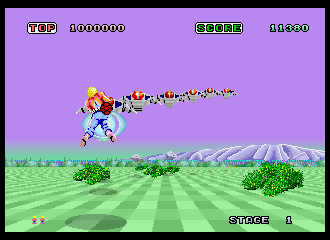
\includegraphics[width=.8\linewidth]{spaceharrier}
  \caption{\textit{Space Harrier} (1985)}
  \label{fig:sfig1}
\end{subfigure}
\begin{subfigure}{.5\textwidth}
  \centering
  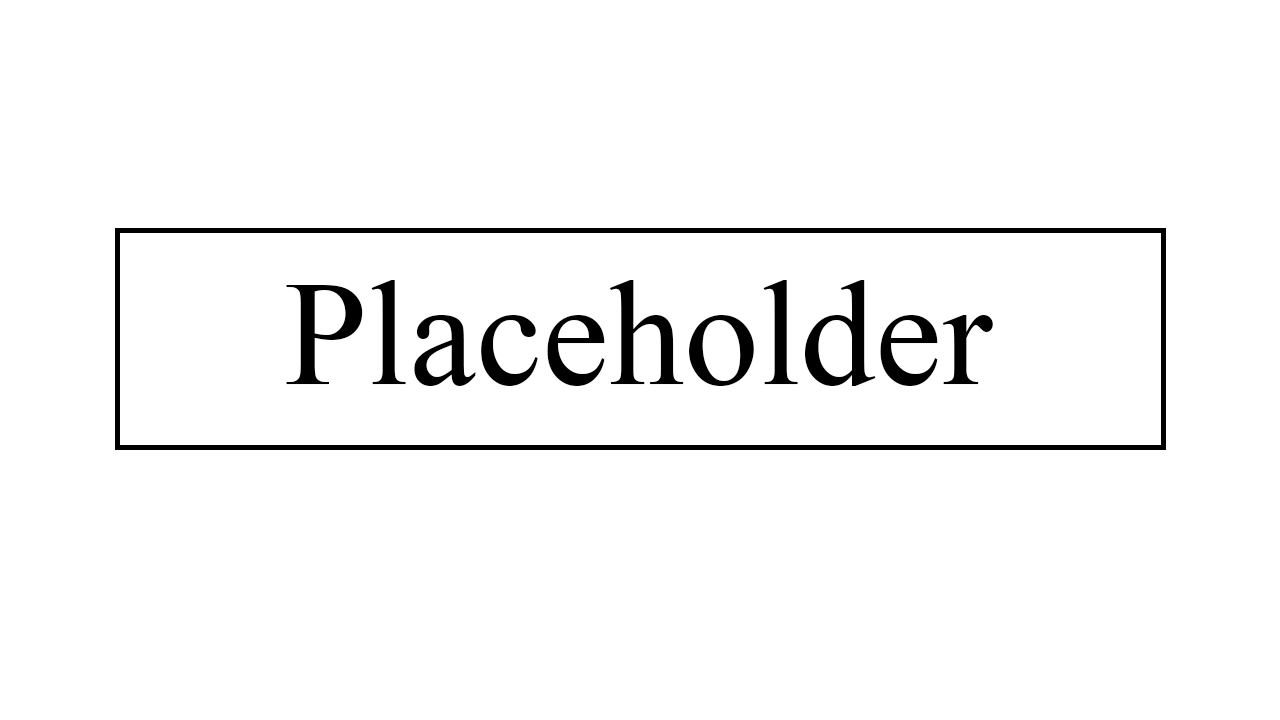
\includegraphics[width=.8\linewidth]{placeholder}
  \caption{\textit{Star Fox} (1993)}
  \label{fig:sfig2}
\end{subfigure}
\begin{subfigure}{.5\textwidth}
  \centering
  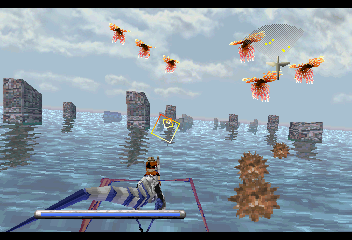
\includegraphics[width=.8\linewidth]{panzerdragoon}
  \caption{\textit{Panzer Dragoon} (1995)}
  \label{fig:sfig3}
\end{subfigure}
\begin{subfigure}{.5\textwidth}
  \centering
  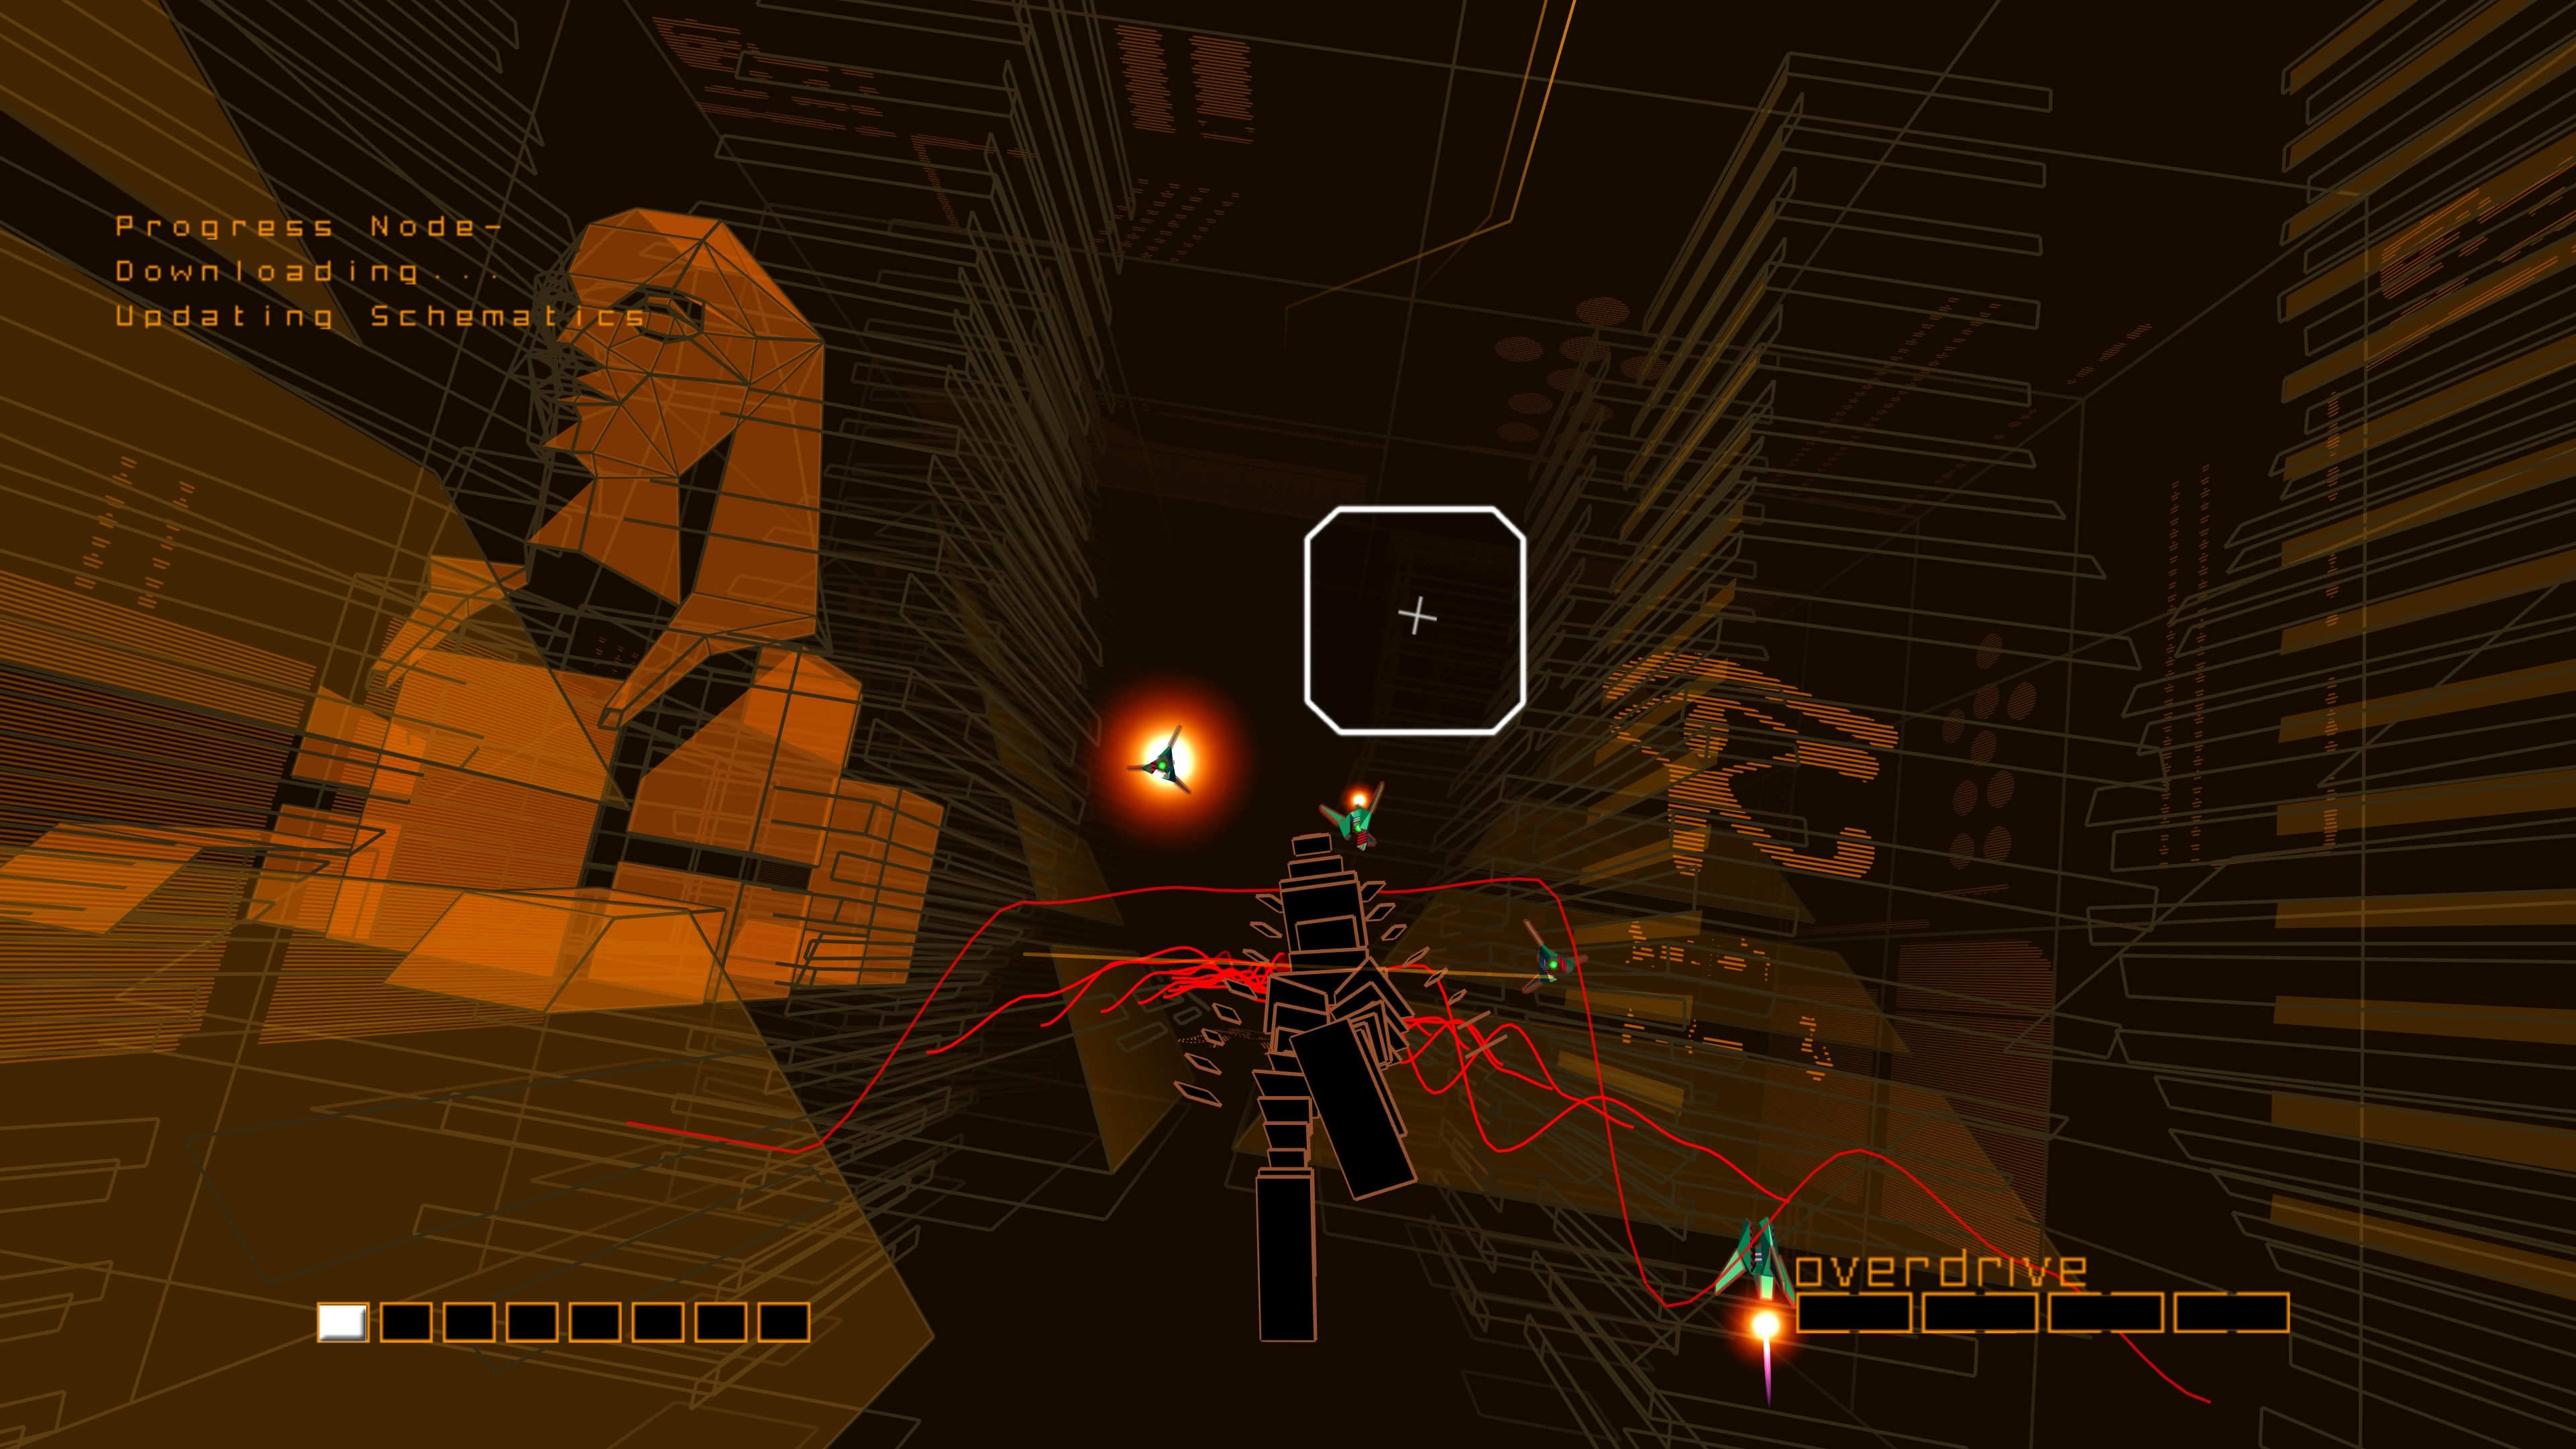
\includegraphics[width=.8\linewidth]{rez}
  \caption{\textit{Rez Infinite} (2016)}
  \label{fig:sfig4}
\end{subfigure}
\caption{four exemplar rail shooters}
\label{fig:history}
\end{figure}

\subsubsection*{Gameplay taxonomy}
% Describe the basic structure of a 3D rail shooter with reference to the above examples,
% outlining their various approaches to core gameplay elements like enemy design, player
% movement, shooting and targetting, significant action set-pieces, and their use of
% fixed perspective or a malleable 3D camera.

Rail shooters have a relatively straightforward gameplay structure, in which players are
automatically carried forward along a fixed path - within which they exercise a fairly
limited range of motion along their relative x-axis and y-axis, and within which they
shoot enemies, and avoid both environmental obstacles and incoming enemy fire. In early instances,
the player moves in a straight line with limited freedom to veer (without gameplay consequence),
while later entries in the genre guided players through more complex spatial compositions incorportating
curves and varied levels of elevation.

These games stand in contrast to games in two other related genres in ways which are illustrative.
They differ from gallery shooting games such as \textit{Virtua Cop} and \textit{Time Crisis}, which
often functioned with a physical gun peripheral, because the player remains in constant motion in
a rail shooter whereas gallery shooting games are generally played from a fixed position in the world
with player movement control typically limited to entering or exiting a form of cover. They also
differ from aerial combat games such as \textit{Ace Combat} for the opposite reason - whereas such
games allow players to navigate their ship freely in 3D space, the rail shooter confines movement to
a fixed plane moving through a scripted path.

Player movement typically doubles up as player aiming too - in early iterations of the genre like
\textit{Space Harrier} and \textit{Star Fox}, movement is tied directly to the player's aim in a
linear fashion, and in later polygonal titles the player directly controls the player's targetting
reticle with player model movement following in an indirect fashion. This differs from modern 3D
game input systems in which player movement and player aiming are controlled independently via dual 
analogue control - this sequence of games were largely developed in tandem with the rise of 3D console
gaming, and largely fell out of fashion before dual analogue input became ubiquitous following the
2000 launch of Sony's PlayStation 2.

% investigate camera controls in PD Orta, PD Remake, and Rez Infinite...

Later games in the cycle did contain rudimentary camera controls, however, with \textit{Panzer Dragoon}
allowing players to rotate the camera in 90 degree incerments using the Sega Saturn's shoulder inputs.
Players were able to see the location of off-camera enemies via a low fidelity radar in the heads up
display, requiring strategic decision making about which of four directions to shoot from.

This degree of freedom did not follow in all subsequent entries in the genre, highlighting the importance
of scripting from a design standpoint - in \textit{Rez} for example, camera rotations around the player
do occur, but without intervention from the player and in order to facilitate scripted action
set pieces that occur from different directions.

% Discuss boss set pieces - eg multisprite enemies in Space Harrier, ship in Dragoon, sphere in Rez
\subsubsection*{Genre pitfalls}
Evidence common criticisms of 3D rail shooters as ``glorified technical demos'' with
limited room for gameplay innovation and discuss their waning significance in
commercial game design - with appropriate counter-examples of cult following for
balance.

Although dedicated commercial rail shooters are now virtually extinct, the gameplay mechanics
do live on in sections of popular games - where players lose free control of player movement
and engage in ``moving shooting galleries''. Some notable examples include \textit{Yakuza Zero}
and \textit{some other game with an on-rails shooting section}

\subsection{PICO-8}\label{pico}

% Brief discussion of decision-making process involved in choosing PICO-8 as tool, with focus on
% project scope, interest in technical implementation details, and 3D modelling demands of building
% such a game in an off-the-shelf 3D game engine ala Unreal or Unity.

One of the initial decisions taken in the project was to settle on an appropriate technology
for building the software. The reasons for choosing PICO-8, and a brief introduction to the
system, will occupy the rest of this section.

The most obvious alternative was to use a fully featured off-the-shelf game engine such as
Unity or Godot. This was rejected at the outset for two principle reasons: firstly, the
use of an existing 3D engine with comprehensive given systems functionality (in, for example,
control and manipulation of 3D cameras and collision detection) would have shifted the focus
of the project away from systems implementation and towards less well defined design issues,
risking scope creep in a time-constrained project; secondly, the use of an existing 3D engine
would have increased expectations in dangerous way with regards to aesthetic fit and finish,
turning the project into an exercise in 3D modelling and texturing; and thirdly, these options 
would have introduced additional burdens in build and portability that are not shared by PICO-8.

The benefits of using off-the-shelf technology is discussed further, and retrospectively, in
Section \ref{engines}.

\subsubsection*{Introduction to PICO-8}
% Discuss ethos of PICO-8 as a ``fantasy console'' and outline its technical
% specification - emphasis on compute power, memory limitations, screen resolution,
% player inputs, and token limits - and indicate some of the implications of these
% constraints on project scope.

Developed by Joseph White, aka zep, and initial released in 2015, PICO-8 is a 
fantasy console modelled on the aesthetic of an 8-bit home console (such as,
for reference, the Nintendo Entertainement System or the Sega Master System).

The system is built around the following key constraints\cite{white}, which replicate
the aesthetic constraints of an 8-bit game console while offering a somewhat more
generous compute capability:

\begin{itemize}
   \item a 128x128 pixel display
   \item a fixed palette of 16 colours
   \item execution of four million virtual instructions per second
   \item a sheet of 128 8x8 sprites
\end{itemize}

% insert table of comparison - PICO vs NES vs MS vs SNES vs MD

Rough comparison of PICO-8 with popular home consoles of the 8-bit era, as
shown in Figure \ref{fig:consolecomparison}, reveals a system with roughly the same
compute power as the Master System and more than twice the compute of the Nintendo
Entertainment System (NES), while having a coarser pixel grid than either and
a more limited colour palette. Note that the emulated 4 MHz CPU of the PICO-8 system
is emulated by allowing four million virtual instructions per second and does not
map neatly to the actual performance of a hardware CPU clocked at 4 Mhz, where more
complex issues of efficient cycle utilisation will be apparent.

\begin{figure}[h]
\begin{center}
\begin{tabular}{r|c|c|c}
      & PICO-8 & Master System\cite{mastersystem} & NES\cite{nes} \\
     \hline
     CPU & 4 Mhz & 4 Mhz & 1.66 Mhz (PAL) \\
     Display & 128 x 128 & 256 x 192 & 256 x 240 \\
     Colour palette & 16 & 64 & 52 \\
\end{tabular}
\end{center}
\caption{PICO-8 compared to 8-bit home consoles}
\label{fig:consolecomparison}
\end{figure}

PICO-8 games are written in the a cut down version of the Lua scripting language -
schewing Lua's standard library and instead implementing a bespoke collection of
global functions. This has several advantages for PICO-8 as a prototyping platform... 
% INSERT REASONS LOL

One oddity of the Lua programming language, particularly from the point of view of
game development, is that it is not a traditional object-oriented programming language
insofar as it does not have classes. Nonetheless, a form of prototype-based object orientation
is possible in the language and is used in the project. As the language's creator Roberto Ierusalimschy
explains\cite[p. 151]{ierusalimschy}, \say{each object may have a prototype, which is a regular object where
the first object looks up any operation that it does not know about. To
represent a class in such languages, we simply create an object to be used
exclusively as a prototype for other objects (its instances). Both classes and prototypes work as a place
to put behavior to be shared by several objects.}

\subsubsection*{PICO-8 as prototyping tool}
% Discuss benefits of using PICO-8 as a tool for rapid creation and iteration of
% game prototypes, compare and contrast to full 3D engines like Unity, Godot and Unreal,
% describe suitability given fixed time constraints of an individual summer
% project, and point to games successfully prototyped in PICO-8 (most notably
% \textit{Celeste}).

PICO-8 has significant advantages as a tool for rapid prototyping, and has been used
effectively as a prototyping tool for commercial game projects - most notably
acclaimed 2018 platformer \textit{Celeste}, which began life in a 2015 PICO-8 game jam.

The principle reasons for its effectiveness as a prototyping tool largely complement the
reasons for not adopting an off-the-shelf game engine, outlined above. Namely: PICO-8
has no complex build process and allows rapid tweaking and iteration; PICO-8 is extremely
portable and, because of its low demand on hardware, performance is guaranteed across a large
range of devices - allowing development to proceed with respect for a known and unchanging
frame budget; and the constraints generated by the system generally prevent scope creep and force
developer focus on essentials.

Additionally, while offering a lightweight development environment without the burdens
imposed by an off-the-shelf engine, PICO-8 does offer a fairly comprehensive suite of
features for getting game projects started quickly - including an \textunderscore update()
and \textunderscore draw()
loop to execute the game, facilities for drawing primitive objects and sprites
to the screen painlessly, simple controls for playing audio across four channels, and
in-built functionality for designing sprites and composing sound effects as shown in Figure
\ref{fig:pico}.

\begin{figure}[h]
\begin{subfigure}{.5\textwidth}
  \centering
  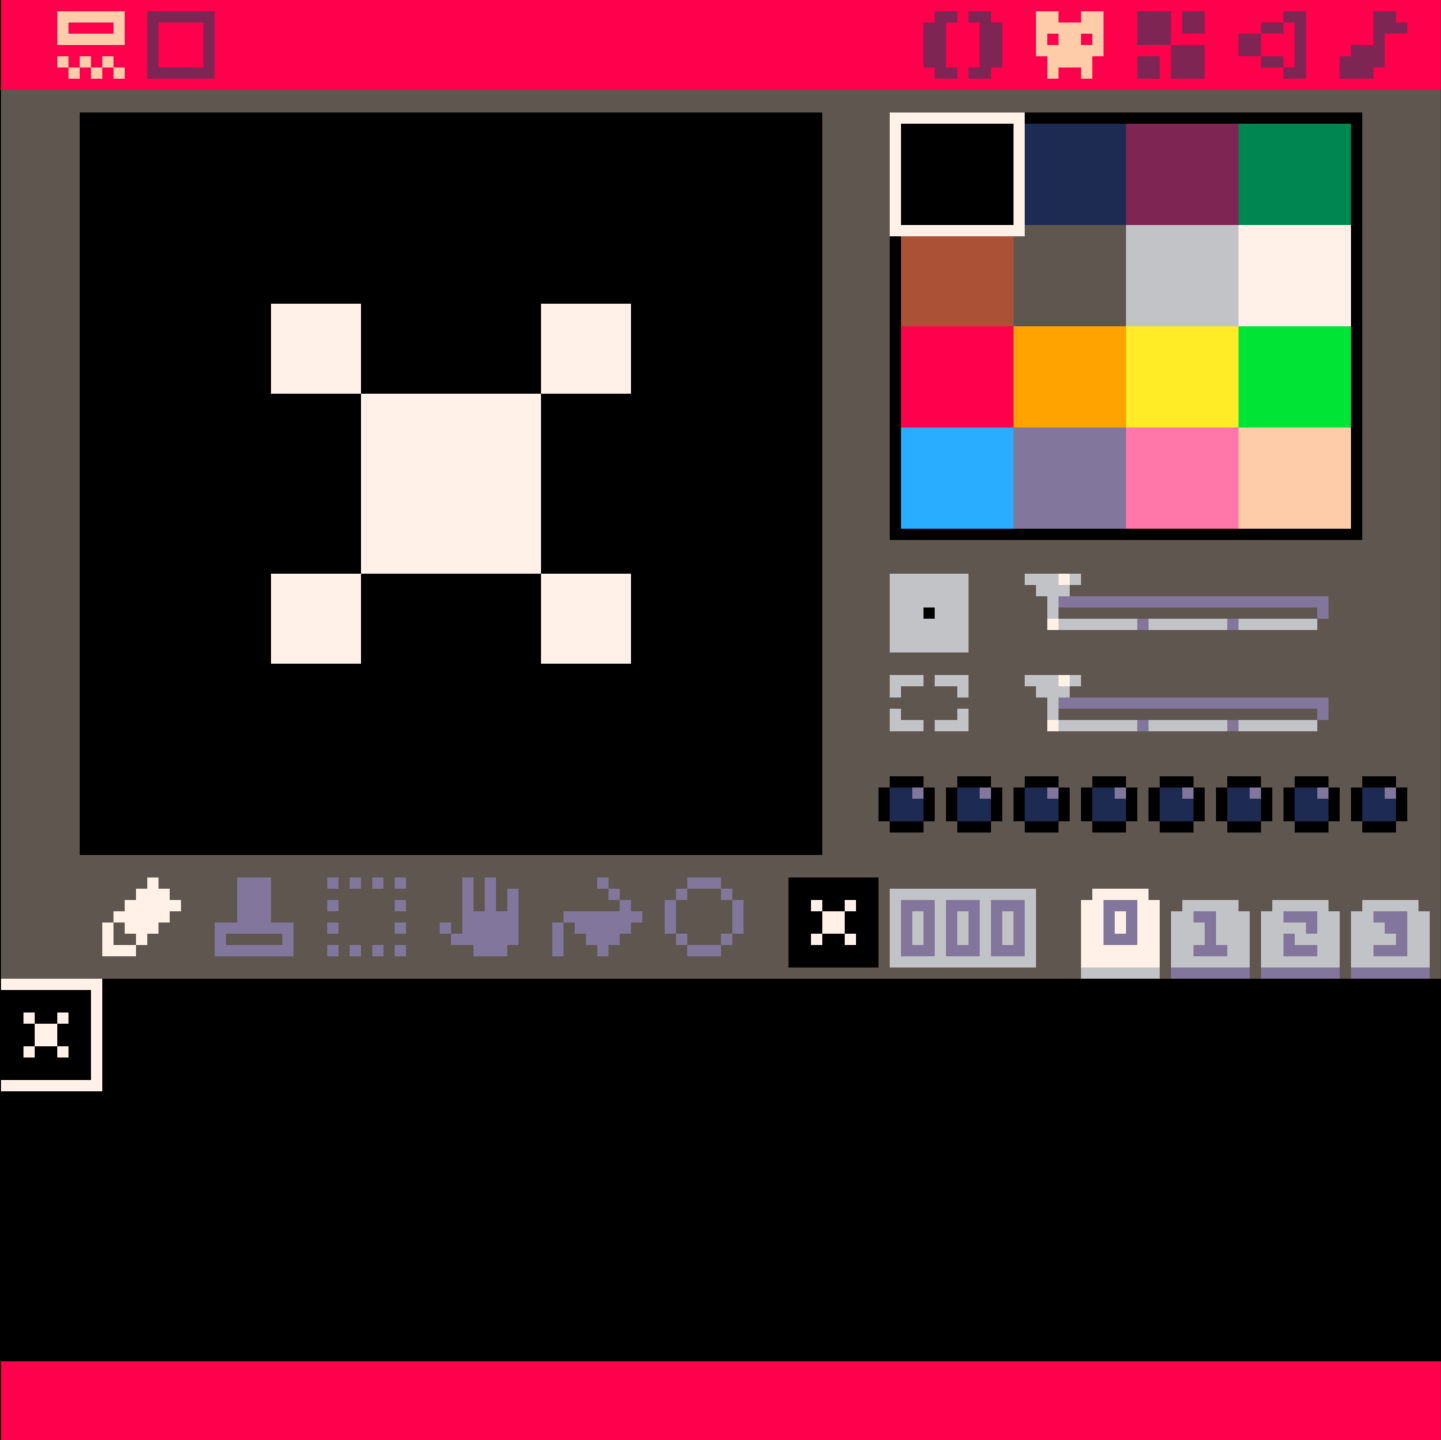
\includegraphics[width=.8\linewidth]{sprite_editor}
  \caption{PICO-8's in-built sprite editor}
  \label{fig:pfig1}
\end{subfigure}
\begin{subfigure}{.5\textwidth}
  \centering
  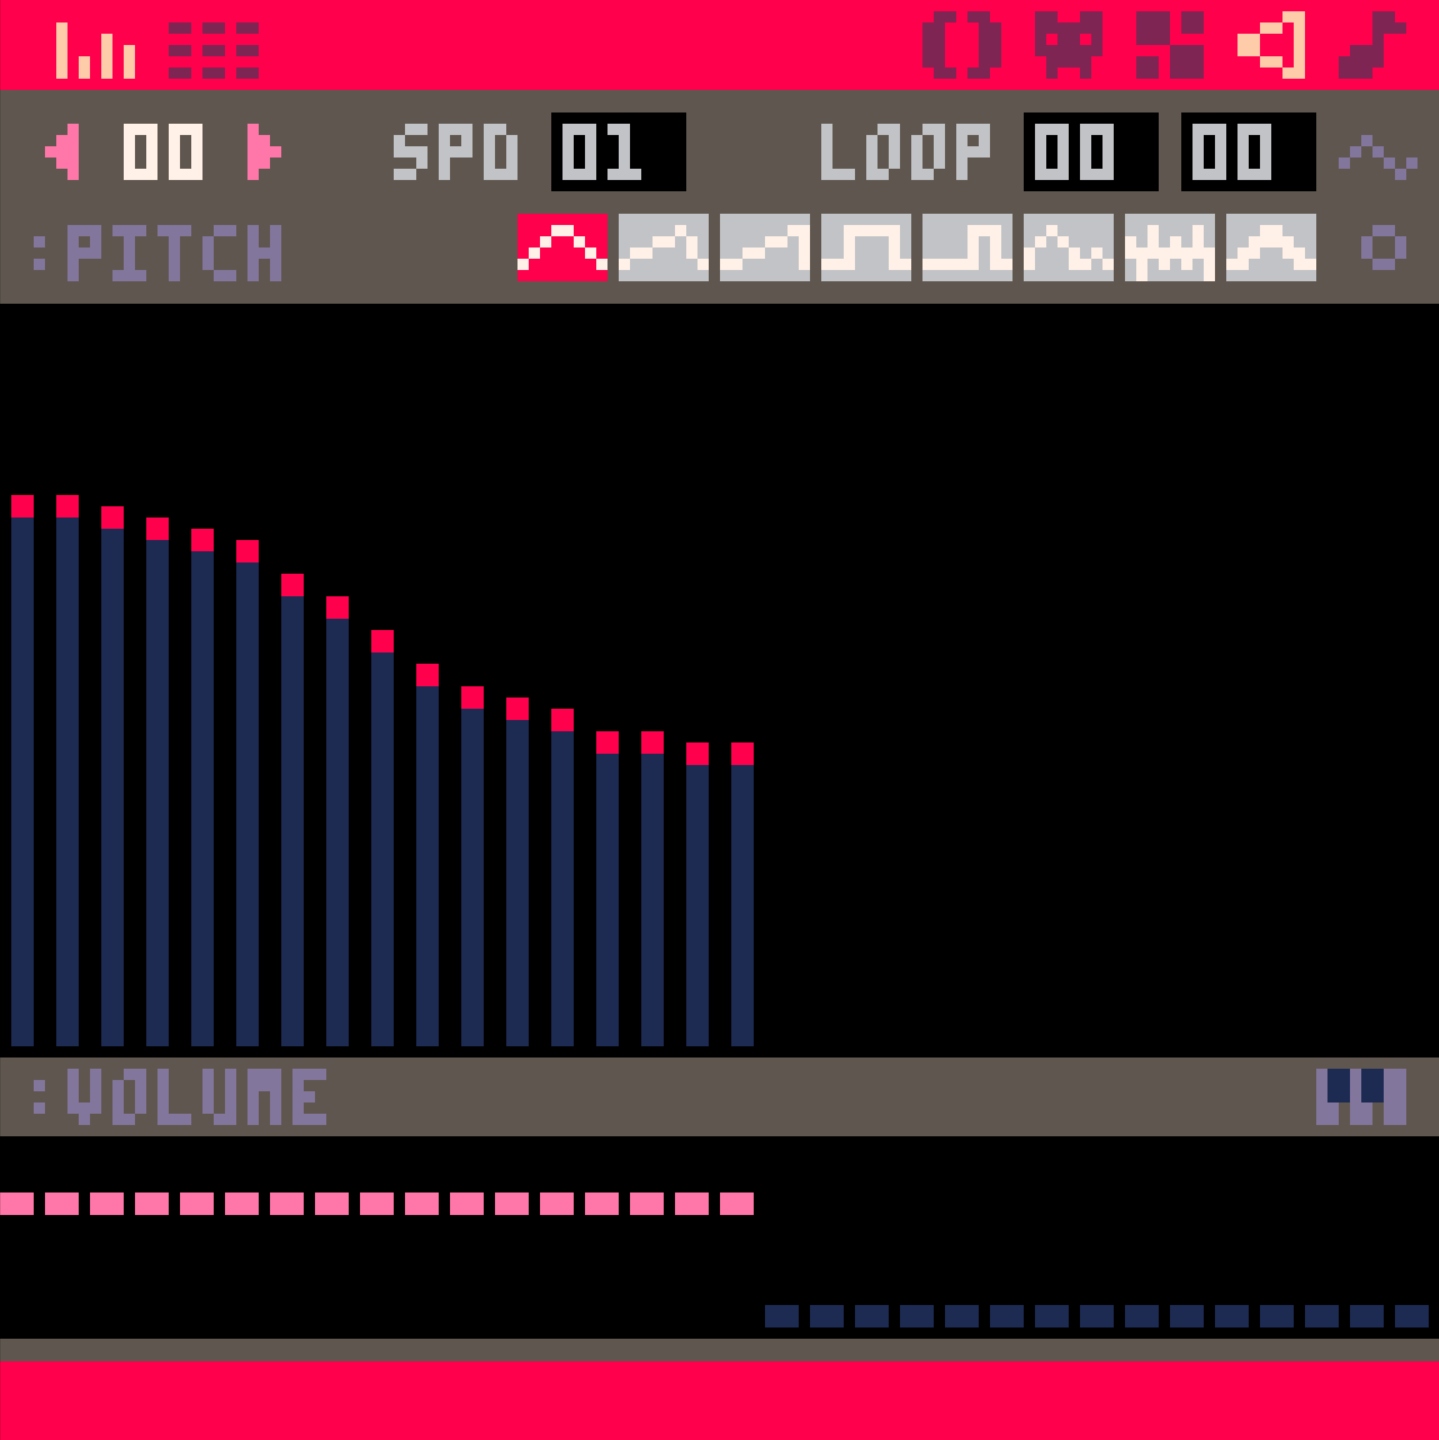
\includegraphics[width=.8\linewidth]{audio_editor}
  \caption{PICO-8's in-built audio editor}
  \label{fig:pfig2}
\end{subfigure}
\caption{PICO-8 asset creation suite}
\label{fig:pico}
\end{figure}

\subsubsection*{Sprite-scaling functionality}
% Discuss PICO-8's given functionality for sprite drawing and scaling and explain how
% these would facilitate development of a low-fidelity game utilising a pseudo-3D
% Super Scaler approach.
One specific advantage of using PICO-8 for this project, in addition to its general
advantages as a prototyping tool, is in-built support not only for drawing sprites
from a sheet but also for dynamically scaling sprites - the core rendering technique
that underlies the early Super Scaler games outlined in Section \ref{genre}.

In addition to the standard sprite drawing call spr() - which is ideally suited to
typical 2D games in which sprites are drawn at a constant size - PICO-8 also offers
an sspr() function that allows the programmer to dynamically scale and stretch sprites
by selecting the extreme corners of a rectangle in screen space into which the sprite
will be deformed and drawn. This, wrapped in functionality to project points in 3D space
to points on a 2D screen, allows the sort of sprite scaling that can simulate depth in 3D
space among multiple 2D sprite assets. This process is described in greater detail in
Section \ref{conversion}.

Where PICO-8 is disadvantaged is in the lack of support for arbitrary rotation of sprites -
a limitation imposed both by PICO-8's effort to emulate 8-bit games systems, which did not yet
have this facility, but also by the coarseness of the platform's pixel grid and the low fidelity
of accompanying sprites which resist easy rotation around small angles. So, whereas late
Super Scaler games like \textit{After Burner} could increase immersion by easily allowing
camera tilting - simulating a degree of aircraft roll in that case - this project will
draw from a more limited set of possibilities in camera control.

\subsubsection*{Extensibility of 2D primatives for 3D}
% Discuss \textit{Star Fox} as exemplar polygonal rail shooter built within similar
% constraints and make critical comparison between PICO-8 platform specification and
% the Super Nintendo with on-cartridge Super FX graphics chip.
One ambition of this project, however, is to go a step beyond sprite scaling effects
and also introduce a limited degree of polygonal rendering - following the example of
Argonaut Software's 1993 Super Nintendo title \textit{Star Fox}, which leveraged bespoke
hardware to drive polygon rendering which is beyond PICO-8 only in scale.

% Discuss extensibility of PICO-8's functions for drawing primitives (eg rectfill and line)
% for triangle rasterisation and polygonal rendering.
Since, at root, polygonal rendering only requires the ability to draw triangles onto a
screen, PICO-8 can therefore perform the requisite functions if given primitive shape calls such
as line() and rectfill() are appropriately extended to draw filled shapes between three points.
The extension of these functions, to draw triangles and render polygonal models composed of
triangles, is discussed in Section \ref{prototyping}.

\subsubsection*{3D experimentation in PICO-8}
Broad overview of existing experimentation with polygonal 3D in PICO-8 with a
focus on \textit{PICO-Fox} as closest analogue. 

Discuss exposed limitations of approach - particularly heavy cost of geometry data
for 3D models, and limitations imposed on design by use of polygonal enemies as
standard (ie minimum size constraint forced by low readability of small 3D models
on a coarse pixel grid).

\subsubsection*{Mitigation strategies for constraints}
Discuss apparent mitigation stategies to work effectively with PICO-8 in light of
the known constraints of the system. Emphasis on:
\begin{itemize}
   \item aggressive use of OOP to eliminate code dupication and preserve token count;
   \item use of standard 30Hz display mode rather than higher-refresh 60Hz mode, to
   trivially double frame budget when drawing and manipulating 3D models;
   \item a blended 2D/3D approach that reserves polygonal rendering for the player
   sprite and for boss encounters, and allows the flexibility and low cost of
   sprite-based gameplay throughout the rest of the core gameplay loop;
   \item possible growth into a ``multicart'' game, in violation of a basic intended
   constraint of the system, as a last resort to deal with token limits.
\end{itemize}

% OOP

One of the most pressing constraints when developing for PICO-8 is the per-cart token
limit, which constrains the amount of code the can define your game. It is therefore
imperitive to practice good discipline in coding, avoiding code duplication and making use
of well structured object-oriented software architecture. PICO-8 carts are written in the
Lua scripting language, which is not traditionally object-oriented but which does have the
facilities to allow a form of prototype-based object orientation using metatables.
% use quotes from the Lua book 

% frame target ?? to keep or to cull...

Another obvious mitigation is to use the console's default 30Hz refresh mode rather than
the optional 60Hz mode. While faster refresh creates a more fluid and responsive game,
it trivially halves your frame budget.

% blended approach

While the project aims to incorporate polygonal rendering, one important mitigation against
PICO-8's constraints is to not dogmatically adopt a purely polygonal approach and instead
opt for a blended approach that uses both polygonal and sprite-based rendering in a
blended way, allowing for more action on screen while allowing perspective-correct 3D models
in situations where they benefit the game.

% multi cart

One further possible mitigation involves eschewing one of the system's constraints entirely.
PICO-8 does allow carts to load and run other carts, allowing developers to sidestep token
limits and build out multi-cart games, in which sections of the game are broken out into
separate discrete carts - perhaps sharing some assets and functionality - and then chained
together using load and run calls.

This approach will be discussed in more detail in Section \ref{multicart}, since it was an
approach ultimately taken in the final stretch of the project.

% Constraints

The choice of technology does also impose constraints that cannot be easily mitigated, and
instead will simply determine aspects of the game's design. As mentioned above, the system
does not have native support for sprite rotation and as such credible camera tilting is simply
not feasible as a technique.

Likewise, the limited number of player inputs (four directions and
two face buttons) minimise the range of actions available to the player - combinations of inputs
(for example, holding B while using directions) would allow us to expand the actions available
to the player, but at an obvious cost to intuition. This constraint can also be seen to
compound with other constraints - for example, a combination of face button and direction
button could facilitate a real-time camera rotation, but the coarseness of PICO-8's pixel
grid would make it difficult to communicate the clear radar information required to
make decisions about camera control meaningful in the first place.

\section{Implementation I: Prototyping}

\subsection{Paper prototyping, software prototyping, and 3D rendering test}\label{prototyping}
The prototyping phase of the project began with three pieces of work along two tracks: firstly,
a paper prototype concretising the core gameplay loop, in which the player moves forward through
space and encounters enemies, and a software implementation of that paper prototype in PICO-8; and
secondly, initial technical work confirming the potential of PICO-8 for polygonal rendering and
allowing me to start getting to grips with the basic ideas behind real-time rendering in general.

\subsubsection*{Basic player actions using primatives}

\begin{figure}[h]
\begin{subfigure}{.5\textwidth}
  \centering
  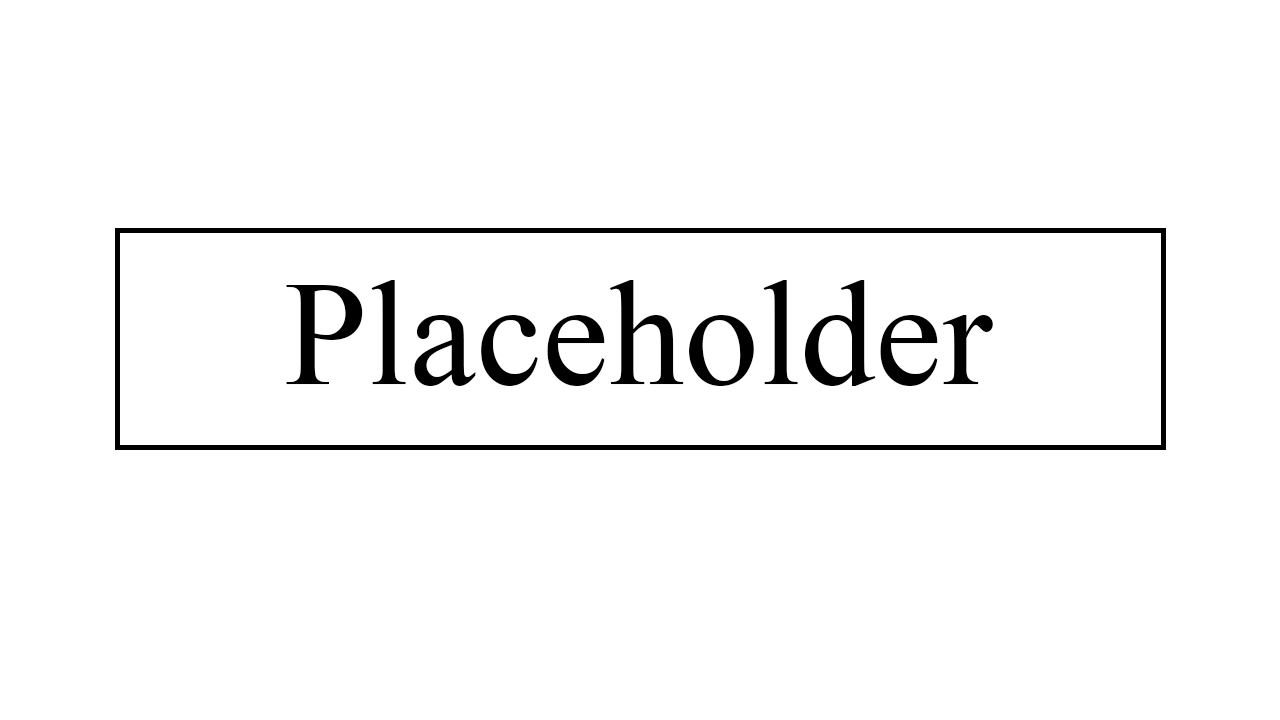
\includegraphics[width=.8\linewidth]{placeholder}
  \caption{paper prototype}
  \label{fig:pfig1}
\end{subfigure}
\begin{subfigure}{.5\textwidth}
  \centering
  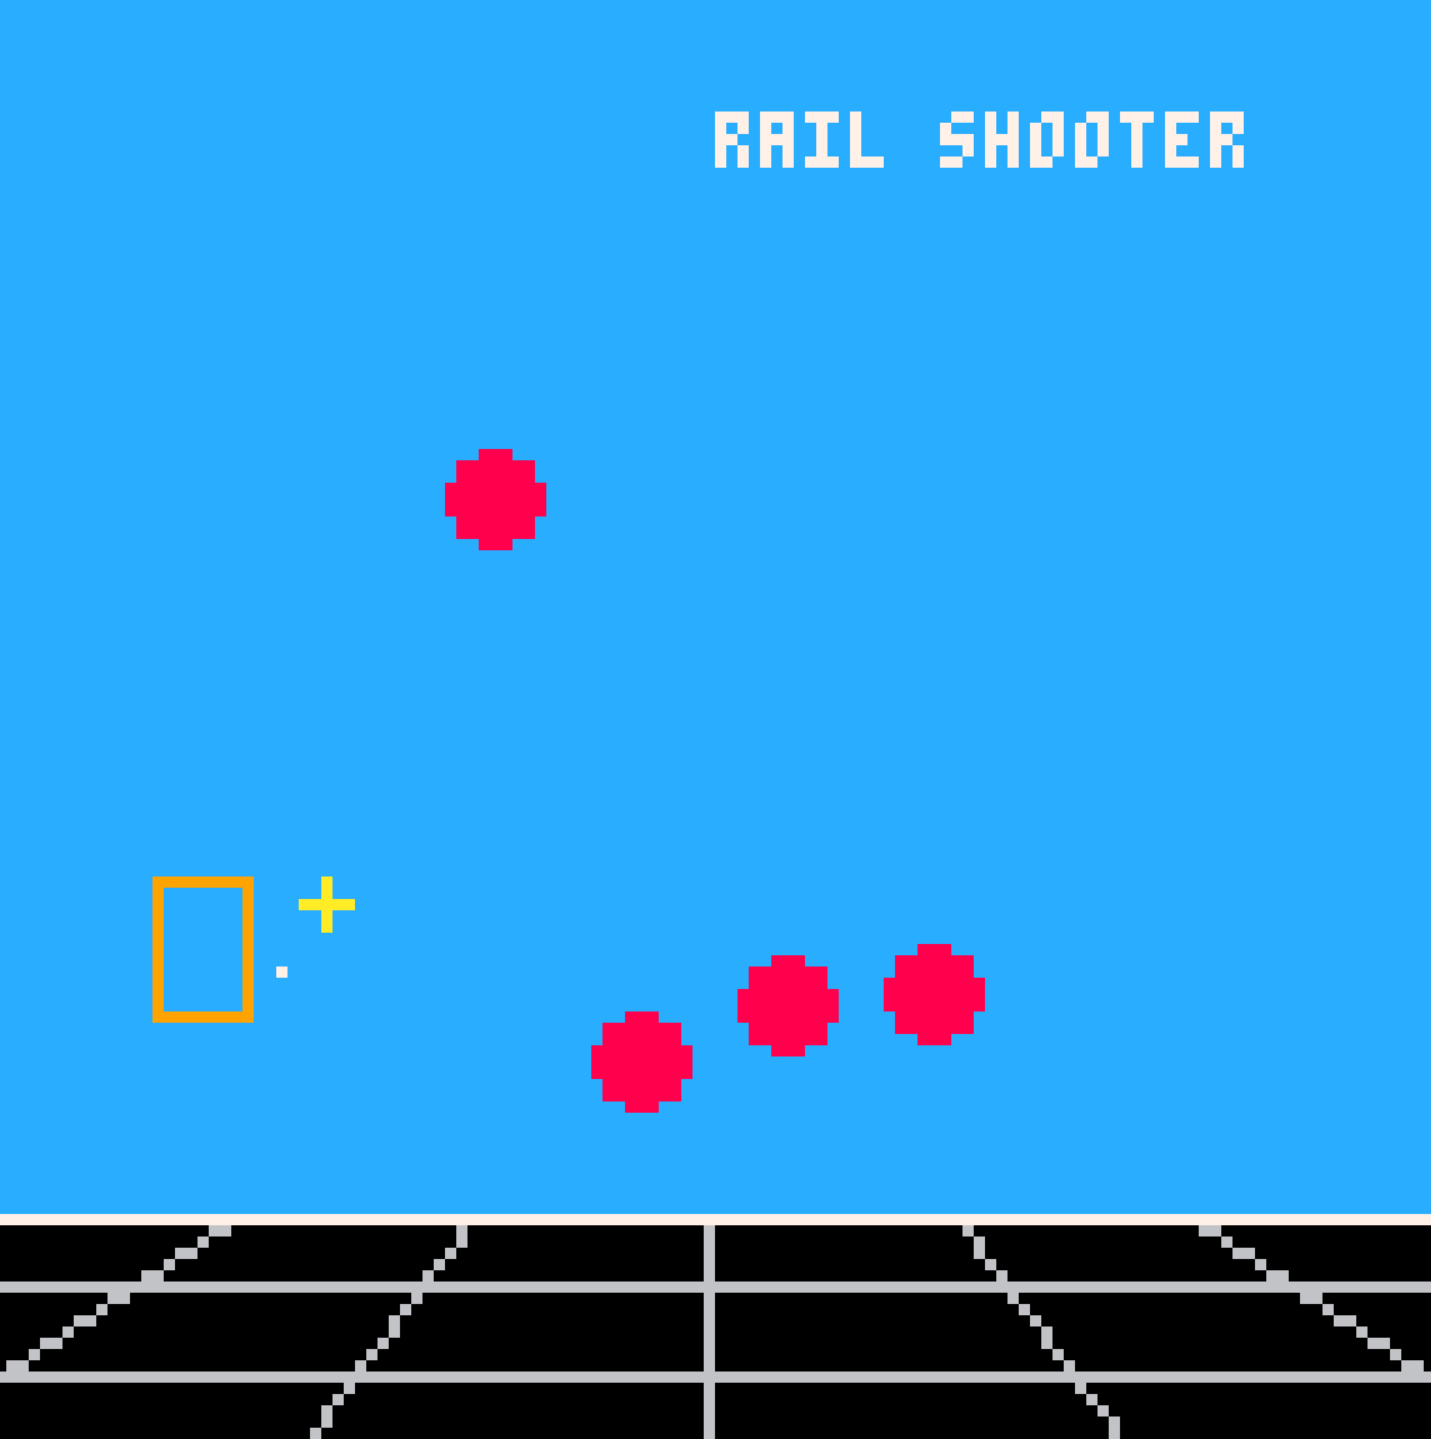
\includegraphics[width=.8\linewidth]{prototype2d}
  \caption{initial software prototype}
  \label{fig:pfig2}
\end{subfigure}
\caption{early prototyping}
\label{fig:gameprototype}
\end{figure}

% Referring back to the gameplay taxonomy conducted in the background section, explain
% how the most significant user actions were distilled down to fit a six-input
% gamepad. Showcase how this was modelled using a flat paper prototype and outline
% how this was translated into a software prototype using primitive shapes to model
% the player and randomly spawned enemies, with movement and interactions being
% directly translated into screen-space.

The primary purpose of the initial paper prototype was to distill the core essence of the
genre, as outlined in the gameplay taxonomy of Section \ref{genre}, into an interactive
medium that allowed easy play with various gameplay elements - examining, for example,
the possible relationships between a player sprite and its firing reticle, and possible
patterns of enemy movement.

Because of the limitations of prototyping on paper, this
phase focused on fairly linear gameplay in which the player moved forward along a straight
path and encountered enemies who existed along a single hypothetical plane in front of
the player, as can be seen in \ref{fig:pfig1}.

Several basic features of the game were explored through this prototype, including the
motion of projectiles in screen space between the player sprite and its reticle, the
motion of enemy projectiles towards the player, and the use of a lock-on mechanic akin to
that implemented in \textit{Panzer Dragoon} and \textit{Rez}.

Following construction of this rudimentary paper prototype, work began on a light software
prototype describing the same basic game behaviours, as seen in \ref{fig:pfig2}, based on the
use of PICO-8's drawing functions for primitive shapes - in this case, rect(), rectfill(),
circfill(), and line().

In this version, the player primarily controls the firing reticle rather than the player sprite,
with the relationship between sprite and reticle defined by their distance from the centre of the
screen - the player reticle is bound to an internal box in screen space, and to create an easy
illusion of depth, the player sprite (here simply a hollow rectangle) is drawn closer to the
real edge of the screen by a linear factor.

Developing out of the paper prototype, much of the logic of this initial software prototype occurs
in screen space, rather than being projected out from a hypothecated 3D world space. Advancing on
the paper prototype, a simple illusion of movement in depth is given to the circular enemy shapes
through naive enlargement in screen space, but bullets still move linearly across the screen instead
of accurately rendering perspective-correct movement through depth.

% Highlight issues already identified at this early stage of prototyping - such as
% player model blocking, the relationship between the player reticle and the destination
% of projectiles in hypothecated 3D space, the need for limitations on enemy
% target locking, and the need for game objects to have a meaningful existence in 3D
% space.

The benefits and pitfalls of paper prototyping for a 3D game project, and its impact on the
direction of the initial software prototype, are discussed further and retrospectively in
Section \ref{prototypepitfalls}.

Briefly, in addition to developing comfort with the basic structure of the game and beginning
to define its basic behaviours, the paper prototype and initial software prototype revealed the
need to start grappling with the design of a correct 3D system, in which objects have positions
in depth as well as along the axes of a screen. This phase of development will be discussed in
Section \ref{conversion}.

\subsubsection*{Simple 3D renderer with model scaling and rotations}

% Describe the contruction of a simple 3D renderer to prove suitability of PICO-8 for
% the proposed project. Expose and discuss my implementation of triangle rasterisation
% in PICO-8 and briefly explain the benefits of decomposing 3D shapes into triangles
% rather than quads. Discuss related issues in polygonal rendering such as triangle
% sorting and backface culling.

While working on the initial software prototype outlined above, a second course of work
was followed to confirm the capacity of PICO-8 to render polygonal models and to begin
building the required functionality over and above PICO-8's primitive drawing functions.

Firstly, a simple algorithm was implemented to draw a filled triangle between three points
in screen space, using line-by-line rect() calls to draw lines between appropriate points on the
sides of the triangle. The rectangular draw function rect() is used
rather than the more intuitive line() function, because PICO-8's implementation of line drawing
includes additional overhead to calculate best fitting lines between diagonal points, even when
drawing lines between two points that share a position on one axis.

Triangles are used as the building block for polygonal rendering because three points, which define
a plane in 3D space, guarantee stable flat surfaces - whereas quad rendering can produce surfaces
between points that are under-described, with a fourth point sitting on a different plane to the
other three and creating ambiguities in the relation of points across a surface. It should be
noted, however, that nothing forces us to use triangles - and indeed the Sega Saturn did render
polygonal graphics using texture mapped quads.

% triangle algorithm

The coordinate points of the triangle are first sorted by their \textit{y}-axis position. The
per-line step required to draw the long side is then calculated by dividing the \textit{x}-axis
distance between the highest and lowest point by their distance in \textit{y}.

The two shorter sides are then calculated by performing the same operation between the highest
and middle points, and again between the middle point and the lowest point. Appropriate logic is
included to handle edge cases too - for example, where two or three points share a position in
\textit{y}.

% point projection

Once triangle drawing functionality was built, functionality to translate 3D coordinates onto
screen space was required. This was done through the use of point projection calculations which
will be discussed in more detail in Section \ref{conversion},
where its broader application to the game software itself will be covered.

% description of 3D models

3D models are described by giving the position of their vertices in 3D model space - that is,
with the object centred around origin (0, 0, 0) so that it can easily be scaled and rotated
before being translated into a more specific world space location. The vertices are then connected
in data defining the triangles they form in the model, with points listed in clockwise order from
the outside to establish their orientation and enable techniques like backface culling.

% discuss scaling and rotation functions

% discuss triangle sorting and backface culling

% PERHAPS include code for triangle drawing and polygonal rendering... hmm... 

% Showcase the results of the ``sanity test'', in which multiple
% cubes are drawn to the screen progressively in order to understand the relative
% computational cost of tracking and drawing 3D geometry in PICO-8 and the feasibility
% of real-time polygonal rendering given system constraints and my existing quality
% of implementation.

Once the core rendering functionality had been built for a single cube, the functionality
was subjected to a simple ``sanity test'' to establish confidence that the performance
cost of polygonal rendering in PICO-8 was not too heavy to preclude its use in the
game.

Using common model space data, nine cubes were defined in our PICO-8 cart with simple inputs
to cycle through the numbers being rendered at any one time. Figure \ref{fig:3dprototype}
outlines the results of the testing with backface culling enabled.

% redo these tests - test with and without backface culling and also test a control where
% cubes do not exist unless they are drawn...

\begin{figure}[h]
\begin{subfigure}{.5\textwidth}
  \centering
  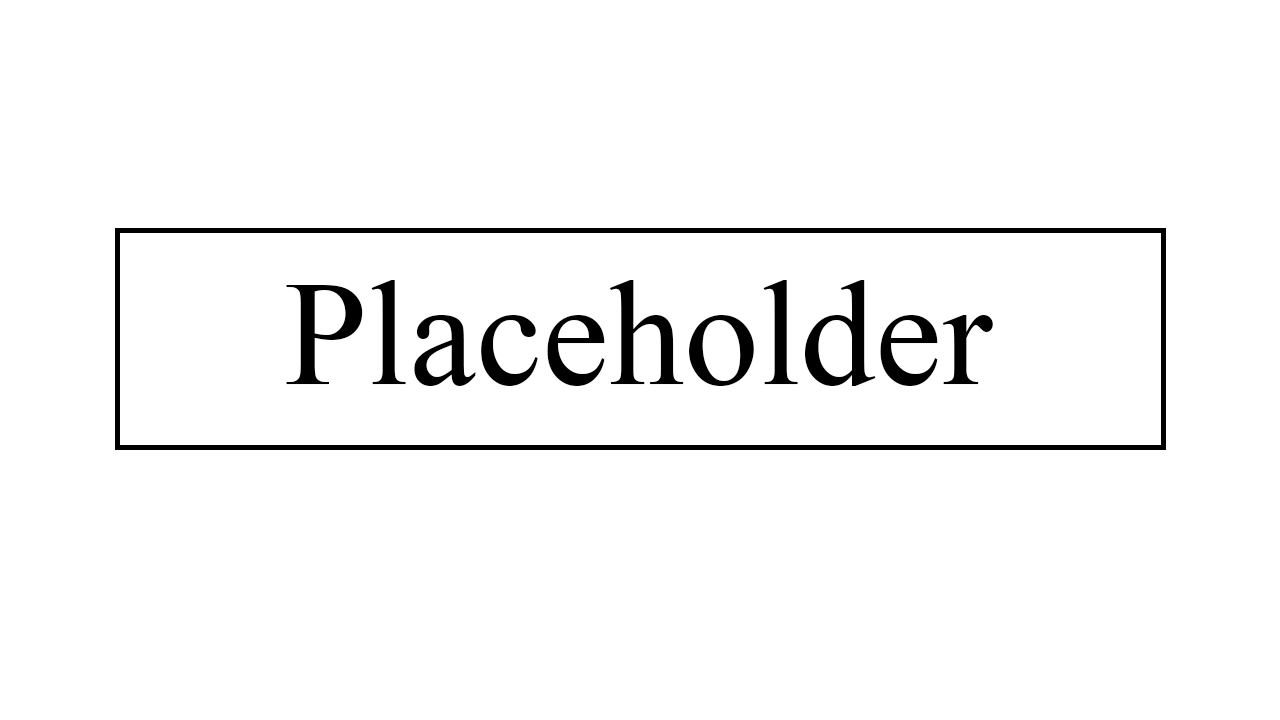
\includegraphics[width=.8\linewidth]{placeholder}
  \caption{single cube render}
  \label{fig:3dfig1}
\end{subfigure}
\begin{subfigure}{.5\textwidth}
  \centering
  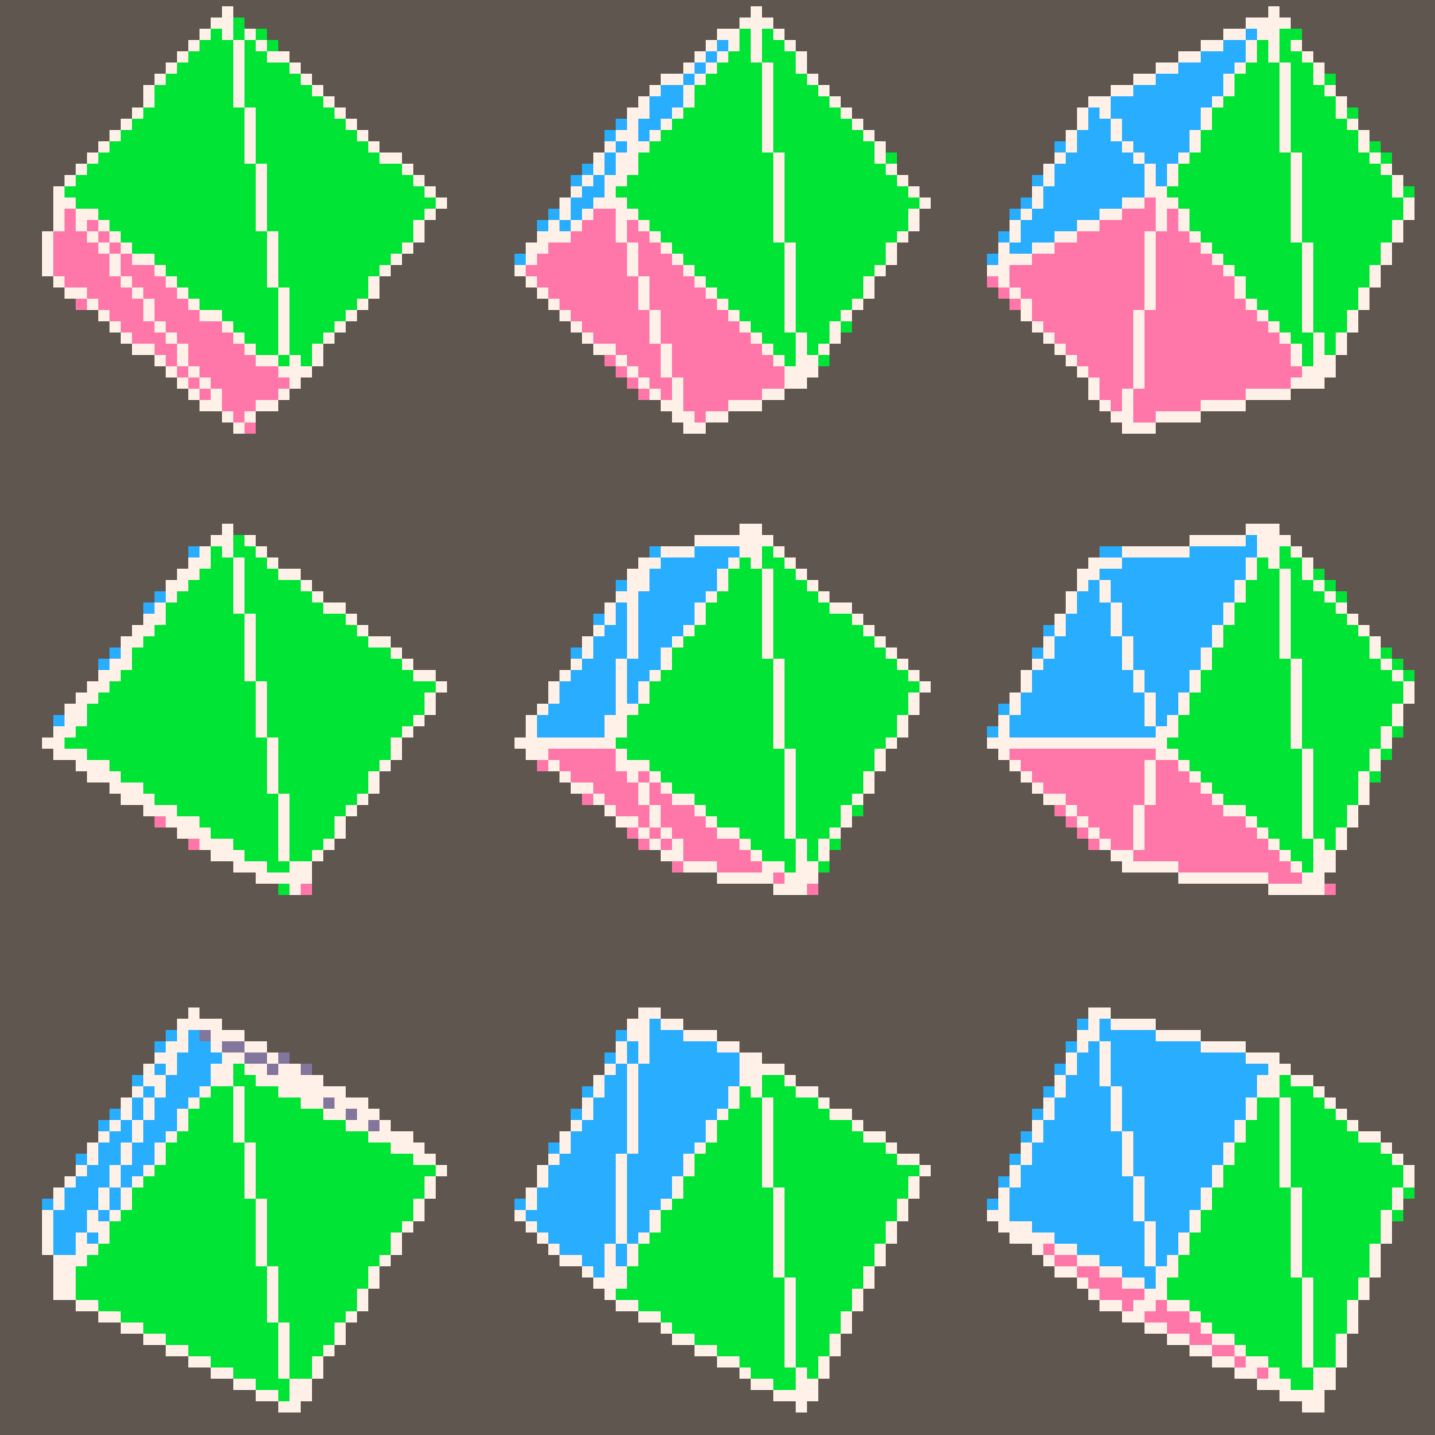
\includegraphics[width=.8\linewidth]{test3d}
  \caption{multi-cube sanity check}
  \label{fig:3dfig2}
\end{subfigure}
\caption{early prototyping}
\label{fig:3dprototype}
\end{figure}

\begin{figure}[h]
\begin{center}
\begin{tabular}{r|c c c c c c c c c c}
     Cubes drawn & 0 & 1 & 2 & 3 & 4 & 5 & 6 & 7 & 8 & 9 \\
     \hline
     CPU utilisation & .37 & .39 & .41 & .43 & .46 & .47 & .49 & .50 & .52 & .53
\end{tabular}
\end{center}
\caption{CPU load sanity testing results}
\label{fig:3dtest}
\end{figure}

\subsection{3D conversion of software prototype}\label{conversion}

While the initial software prototype served a useful purpose in creating familiarity
with the basic mechanics and feel of the game, and sparking early thinking about some of the
significant design decisions that needed to be made, its origins in a flat paper prototype
also led to key technical implimentation issues being elided - namely the accurate handling
of depth and perspective necessary to properly deliver on the initial idea of the project.

As such, the initial software prototype was built on in the next phase of development and refactored
so that objects carried proper three-dimensional positions in world space, and were drawn in a
properly scaled and perspective correct way instead of having movement in depth faked through
arbitrary re-scaling in screen space. Likewise, collision handling was re-written to accurately detect
intersections of bounding volumes in three-dimensional space, instead of being handled through
screen space intersection in a 2D plane.

\subsubsection*{Perspective-correct 3D projection and scaling}
% Discuss the application of 3D point projection to the corners of 2D sprite objects
% to achieve perspective correct drawing and scaling of 2D elements using PICO-8's sspr
% function. Highlight use of small camera movements (spatial displacement in x and y)
% aligned to player sprite movement to heighten illusion of depth along the z-axis.
One of the key changes introduced in this 3D software prototype was the creation of accurate
depth among enemy units, created by correctly projecting sprite objects onto the screen using
newly introduced \textit{z}-coordinate values.

In order to accurately project a point from 3D space onto a screen, we must hypothecate a viewport in 3D space
and a camera position, and then exploit the law of similar triangles to identify the point in space at
which the the line between the point and our camera - which will be positioned at at the origin of the
coordinate system, (0, 0, 0), for simplicity - intersects with our viewport.

\begin{figure}
   \centering
   \begin{tikzpicture}
      [scale = 1.5,
      axis/.style={-stealth},
      dot/.style= {
         draw,
         fill = black,
         circle,
         inner sep = 0pt,
         minimum size = 4pt
      },
      point/.style= {
         draw,
         fill = black,
         circle,
         inner sep = 0pt,
         minimum size = 2pt
      }]
      
      \draw[axis] (-0.5, 0) -- (5, 0) node[right] {$z$};
      \draw[axis] (0, -0.5) -- (0, 2) node[above] {$y$};
      \draw (1, -0.25) -- (1, 1.5) node[above] {$viewport$};

      \draw (3, 1.5) node[dot, label = {right:$P$}] {};
      \draw (3, 1.5) -- (3, 0);
      \draw (3, 1.5) -- (0, 0);

      \draw (0, 0) node[below left] {$O$};
      \draw (1, 0) node[below left] {$A$};
      \draw (3, 0) node[below] {$B$};
      \draw (1, 0.5) node[dot, label = {above left:$P'$}] {};

   \end{tikzpicture}
   \caption{side orthographic view of a point projection on the \textit{y}-axis, adapted from figure 9-2 of Gambetta
   \cite[p. 106]{gambetta}}
   \label{fig:triangles}
\end{figure}

This operation must be performed along both the \textit{x} and \textit{y} axes, and figure \ref{fig:triangles}
illustrates how the law of similar triangles can be used to determine viewport projection of point \textit{P}
in the \textit{y}-axis as an example. \cite[p. 106]{gambetta}

Because triangles OBP and OAP' are similar triangles - that is, they are right angled triangles that have the same
internal angles - we can leverage the fact that, as similar triangles, the ratio of their equivalent sides is the same.

Therefore we can say that the ratio of lengths OA and AP' is the same as the ratio of lengths OB and BP. If we know
the coordinate position of point P, we know that OB is its position in \textit{z} and BP is its position in \textit{y}.
We also know that length OA is simply the distance between the camera and the viewport - a distance which we know because
we have hypothecated these objects in 3D space ourselves. As a consequence, the length of the line AP' is:

\begin{equation}
   |AP'| = \frac{|BP| * |OA|} {|OB|}
\end{equation}

or, the \textit{y} coordinate of the point, projected onto the viewport V, is:

\begin{equation}
   V_y = \frac{P_y * V_z} {P_z}
\end{equation}

Once this calculation is made, we simply need to translate the figures for our actual screen or canvas, which uses different
measures from our in-scene viewport, and this is achieved by multiplying the calculated coordinate by the width or height of
our canvas in pixels (128 in both axes in PICO-8), and dividing this by the in-scene width or height of our viewport.

In figure \ref{fig:equationsproject} we see how this calculation can be simplified by hypothecating a 1 by 1 in-scene viewport and
a viewport distance of 1 in \textit{z} - since any number divided or multiplied by 1 remains unchanged, we can simply eliminate
arbitrary multiplications and divisions from our computation and scale our scenes for this set-up. The downside of this approach,
however, is that it does lock us into a particular field of view.

Finally, the position value must be adjusted to account for the fact that the centre of our in-scene viewport looks directly
along the \textit{z}-axis along \textit{x}, \textit{y} coordinates of (0, 0), whereas (0, 0) on our canvas exists
in the top left corner of the screen rather than the centre, and the positive direction of \textit{y} is therefore
inverted on our screen too.

This entire operation is implemented in the code highlighted in figure \ref{fig:codeproject} using a single short function
that takes a three-component vector - representing the \textit{x}, \textit{y}, and \textit{z} coordinates of a
vertex in space - and projects them onto a viewport of width and height 1, centred around (0, 0) and located
one unit along the \textit{z}-axis. This returns two values, for screen projection in \textit{x} and \textit{y}.

\begin{figure}[h]
   \begin{subfigure}{.45\textwidth}
   \centering
      \begin{equation}
         C_x = \frac{\frac{P_x * V_z} {P_z} * C_w} {V_w}
      \end{equation}
      \begin{equation}
         C_y = \frac{\frac{P_y * V_z} {P_z} * C_h} {V_h}
      \end{equation}
   \caption{complete projection equations}
   \label{fig:equationfullproject}
   \end{subfigure}\hfill
   \begin{subfigure}{.45\textwidth}
   \centering
      \begin{equation}
         C_x = \frac{P_x} {P_z} * C_w
      \end{equation}
      \begin{equation}
         C_y = \frac{P_y} {P_z} * C_h
      \end{equation}
   \caption{simplified projection equations}
   \label{fig:equationsimpleproject}
   \end{subfigure}\hfill
\caption{simplification of perspective projection calculations through use of values of 1 for viewport width
and height ($V_w$ and $V_h$), and viewport depth $V_z$}
\label{fig:equationsproject}
\end{figure}

This function is called twice for each sprite drawn, finding the position of the top-left and bottom-right
corners of its face - derived from an object's position, its width, and its height - and then drawing the
sprite using PICO-8's in-built scaled sprite function sspr(), discussed in Section 2.2.

Figure \ref{fig:projection} illustrates how this process renders scenes using perspective projection.
While it highlights the use of this function to project the extreme corners of 2D sprites onto a screen,
the same method is also used by the program to project the three vertices of triangles onto screen space
too - allowing the rendering of polygonal shapes such as the player ship and the icosahedral boss enemy shell,
or the polygonal cubes discussed in the previous section. Discussion of \textit{z}-sorting to ensure proper
ordering as well as proper scaling of objects will be picked up in Section 4.3.

\begin{figure}[h]
   \begin{lstlisting}
project_vert = function(vect3)

   return 64 + (((vect3[1] - camera.x) / vect3[3]) * 128),
           64 - (((vect3[2] - camera.y) / vect3[3]) * 128)

end
   \end{lstlisting}
   \caption{vertex projection function}
   \label{fig:codeproject}
\end{figure}

Note: in the implementation highlighted in figure \ref{fig:codeproject} from the software prototype, displacements
in the \textit{x} and \textit{y} axes were added to represent relative motion of the camera - although this
effect was later removed from the final version of the game, since it tended to make the gameplay harder to reason
about spatially.

\begin{figure}[h]
\begin{subfigure}{.3\textwidth}
   \centering
   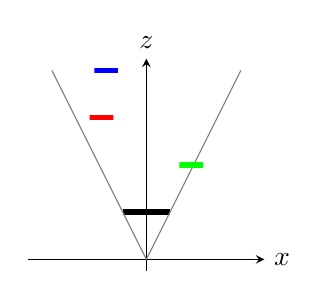
\begin{tikzpicture}
      [scale = .6,
      axis/.style={-stealth},
      dot/.style= {
         draw,
         fill = black,
         circle,
         inner sep = 0pt,
         minimum size = 4pt
      },
      point/.style= {
         draw,
         fill = black,
         circle,
         inner sep = 0pt,
         minimum size = 2pt
      }]
      
      \draw[axis] (-2.5, 0) -- (2.5, 0) node[right] {$x$};
      \draw[axis] (0, -0.25) -- (0, 4.25) node[above] {$z$};

      \draw[line width = 2] (-0.5, 1) -- (0.5, 1);
      \draw[draw = gray] (0, 0) -- (-2, 4);
      \draw[draw = gray] (0, 0) -- (2, 4);

      \draw[line width = 2, draw = blue] (-1.1, 4) rectangle (-0.6, 4);
      \draw[line width = 2, draw = red] (-1.2, 3) rectangle (-0.7, 3);
      \draw[line width = 2, draw = green] (0.7, 2) rectangle (1.2, 2);

   \end{tikzpicture}
   \caption{top orthographic view of a game scene}
   \label{fig:rotfig1}
\end{subfigure}\hfill
\begin{subfigure}{.3\textwidth}
   \centering
   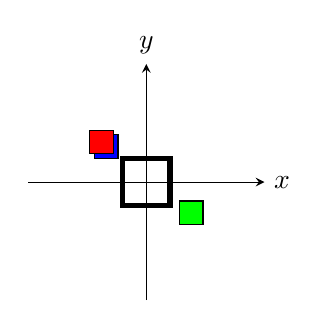
\begin{tikzpicture}
      [scale = .6,
      axis/.style={-stealth},
      dot/.style= {
         draw,
         fill = black,
         circle,
         inner sep = 0pt,
         minimum size = 4pt
      },
      point/.style= {
         draw,
         fill = black,
         circle,
         inner sep = 0pt,
         minimum size = 2pt
      }]
      
      \draw[axis] (-2.5, 0) -- (2.5, 0) node[right] {$x$};
      \draw[axis] (0, -2.5) -- (0, 2.5) node[above] {$y$};

      \draw[fill = blue] (-1.1, 1) rectangle (-0.6, 0.5);
      \draw[fill = red] (-1.2, 1.1) rectangle (-0.7, 0.6);
      \draw[fill = green] (0.7, -0.4) rectangle (1.2, -0.9);
      \draw[line width = 2] (-0.5, -0.5) rectangle (0.5, 0.5);

   \end{tikzpicture}
   \caption{front orthographic view of a game scene}
   \label{fig:rotfig1}
\end{subfigure}\hfill
\begin{subfigure}{.3\textwidth}
   \centering
   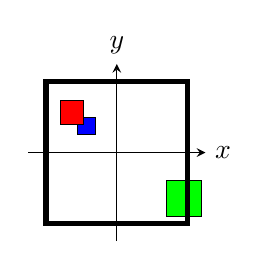
\begin{tikzpicture}
      [scale = 1.8,
      axis/.style={-stealth},
      dot/.style= {
         draw,
         fill = black,
         circle,
         inner sep = 0pt,
         minimum size = 4pt
      },
      point/.style= {
         draw,
         fill = black,
         circle,
         inner sep = 0pt,
         minimum size = 2pt
      }]
      \draw[axis] (-0.625, 0) -- (0.625, 0) node[right] {$x$};
      \draw[axis] (0, -0.625) -- (0, 0.625) node[above] {$y$};

      \draw[fill = blue] (-0.275, 0.25) rectangle (-0.15, 0.125);
      \draw[fill = red] (-0.4, 0.367) rectangle (-0.233, 0.2);
      \draw[fill = green] (0.35, -0.2) rectangle (0.6, -0.45);

      \draw[line width = 2] (0.5, 0.5) rectangle (-0.5, -0.5);


   \end{tikzpicture}
   \caption{perspective-correct projection of sprite objects onto screen}
   \label{fig:rotfig2}
\end{subfigure}\hfill
\caption{projection of a sprite objects in 3D space onto a canvas}
\label{fig:projection}
\end{figure}

\subsubsection*{Real-time 3D collisions}

% Discuss implementation of cuboid bounding volumes to test for collisions, using
% height, width, and depth data paired if three-dimensional positions to check for
% intersection of volumes. Discuss the need for axis-alignment to significantly
% simplify calculations, and the design implications of this with regard to rotational
% symmetry of objects depicted (ie disc-shaped saucers, and spherical projectiles)

Having translated the game into 3D world space for the purposes of perspective-correct rendering, adjusting
the game's collision system was the next logical step.

In the initial software prototype, without \textit{z} values to work with, single pixel projectiles were simply
fired across the screen in a 2D plane with simple checks to see if they had entered the player (represented in
the initial prototype as a hollow rectangle) or enemies (represented as solid circles). This became untenable
as a solution, given that it jarred with perspective-correct rendering of enemy units, and the prototype was
updated to test for collisions using cuboid bounding volumes.

Cuboid bounding volumes can have two principal uses in a collision detection system. In complex simulations,
checks for intersection between cuboid volumes can be used as a pruning mechanism - an initial approximation
to either disconfirm that intersection has occurred, or else call for a more complex test of the actual
geometry being bounded. In more simple systems, such as the low-fidelity game being built in this project,
cuboid volumes can be used effectively to test for collisions in general.\cite[p. 75]{ericson}

Two of the most desirable characteristics of bounding volumes are tightness of fit with underlying geometry,
and ease of rotation and transformation.\cite[p. 76]{ericson} As such, an early design decision was made to
populate the game with objects that are exactly (or close to exactly) rotationally symmetrical.

Therefore projectiles are depicted as spheres, rather than taking on a tapered bullet-shaped appearance. The main
enemy units are depicted as round flying saucers. Both objects can be represented in collision space in
axis-aligned cuboid bounding volumes that do not need to rotate at all to reflect any putative rotation of
the object in space, significantly simplifying intersection calculations.

Although these bounding volumes are not perfect matches for the objects being represented, they are sufficiently
tightly bound to simulate a plausible system of collisions - to quote Christer Ericson, veteran programmer of Sony
Santa Monica and NeverSoft, ``in games, collision detection and response can effectively be governed by `if it looks
right, it is right.' Other applications have stricter accuracy requirements.''\cite[p. 12]{ericson}

\begin{figure}[h]
\centering
\begin{subfigure}{.45\textwidth}
   \centering
   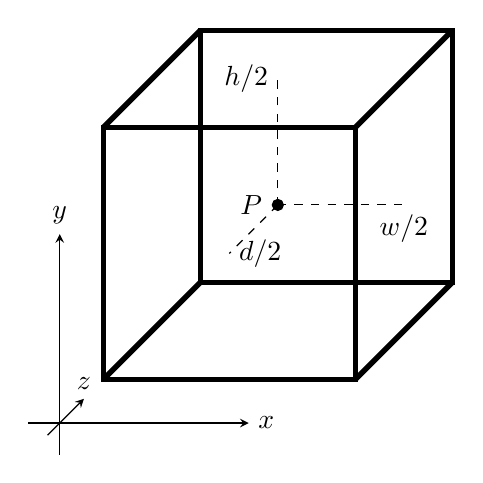
\begin{tikzpicture}
      [scale = 0.8,
      axis/.style={-stealth},
      dot/.style= {
         draw,
         fill = black,
         circle,
         inner sep = 0pt,
         minimum size = 4pt
      },
      point/.style= {
         draw,
         fill = black,
         circle,
         inner sep = 0pt,
         minimum size = 2pt
      }]
      
      \draw[axis] (-0.5, 0, 0) -- (3, 0, 0) node[right] {$x$};
      \draw[axis] (0, -0.5, 0) -- (0, 3, 0) node[above] {$y$};
      \draw[axis] (0, 0, 0.5) -- (0, 0, -1) node[above] {$z$};

      \draw[line width = 2] (0.5, 4.5, -0.5) rectangle (4.5, 0.5, -0.5);
      \draw[line width = 2] (0.5, 4.5, -4.5) rectangle (4.5, 0.5, -4.5);
      \draw[line width = 2] (0.5, 4.5, -0.5) -- (0.5, 4.5, -4.5);
      \draw[line width = 2] (0.5, 0.5, -0.5) -- (0.5, 0.5, -4.5);
      \draw[line width = 2] (4.5, 4.5, -0.5) -- (4.5, 4.5, -4.5);
      \draw[line width = 2] (4.5, 0.5, -0.5) -- (4.5, 0.5, -4.5);

      \draw (2.5, 2.5, -2.5) node[dot, label = {left:$P$}] {};
      \draw [dashed] (2.5, 2.5, -2.5) -- (4.5, 2.5, -2.5) node[below] {$w/2$};
      \draw [dashed] (2.5, 2.5, -2.5) -- (2.5, 4.5, -2.5) node[left] {$h/2$};
      \draw [dashed] (2.5, 2.5, -2.5) -- (2.5, 2.5, -0.5) node[right] {$d/2$};

   \end{tikzpicture}
   \caption{a centre-radius bounding representation defined by position \textit{P}, height \textit{h},
   width \textit{w}, and depth \textit{d}}
   \label{fig:colfig1}
\end{subfigure}\hfill
\begin{subfigure}{.45\textwidth}
   \centering
   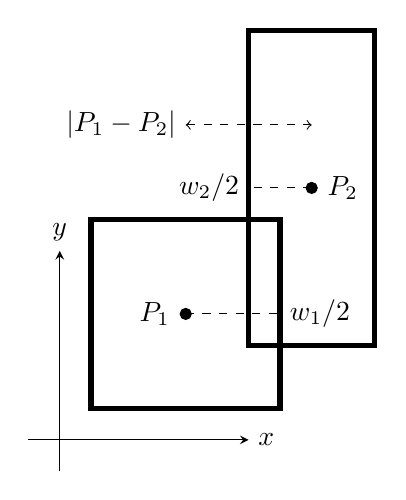
\begin{tikzpicture}
      [scale = 0.8,
      axis/.style={-stealth},
      dot/.style= {
         draw,
         fill = black,
         circle,
         inner sep = 0pt,
         minimum size = 4pt
      },
      point/.style= {
         draw,
         fill = black,
         circle,
         inner sep = 0pt,
         minimum size = 2pt
      }]
      
      \draw[axis] (-0.5, 0) -- (3, 0) node[right] {$x$};
      \draw[axis] (0, -0.5) -- (0, 3) node[above] {$y$};

      \draw[line width = 2] (0.5, 0.5) rectangle (3.5, 3.5);
      \draw (2, 2) node[dot, label = {left:$P_1$}] {};
      \draw[line width = 2] (3, 1.5) rectangle (5, 6.5);
      \draw (4, 4) node[dot, label = {right:$P_2$}] {};

      \draw [dashed] (2, 2) -- (3.5, 2) node[right] {$w_1/2$};
      \draw [dashed] (4, 4) -- (3, 4) node[left] {$w_2/2$};
      \draw [dashed, <->] (2, 5) node[left] {$|P_1-P_2|$} -- (4, 5);

   \end{tikzpicture}
   \caption{front orthographic projection of an intersection check of two volumes, showing comparison along a single axis}
   \label{fig:colfig2}
\end{subfigure}\hfill
\caption{collision of axis-aligned cuboid bounding volumes}
\label{fig:collision}
\end{figure}

Since the game records the position of game objects through a single three-coordinate vector at the object's
centre, axis-aligned bounding volumes use a centre-radius representation\cite[p. 78]{ericson}, as seen in
figure \ref{fig:colfig1}, in which the bounds of the volume are defined by positional data and values for the
object's height, width, and depth - of which height and width are already used for rendering.

Collisions between objects of this representation are then calculated using a simple series of checks comparing
the absolute distance between the objects on each axis by the difference of their radius along that axis as
depicted in figure \ref{fig:colfig2} - here derived as the sum of their relevant extensions divded by two as
outlined in figure \ref{fig:colequation} and implemented in code in figure \ref{fig:codecollide}.

\begin{figure}
   \centering
   Intersection occurs where:
   \begin{equation}
      |P_1 - P_2| < \frac{e_1 + e_2} {2}
   \end{equation}
   in the \textit{x}, \textit{y}, and \textit{z}-axes, where $P_1$ and $P_2$ are an object's coordinates on a given axis and
   $e_1$ and $e_2$ are corresponding values representing the object's extension along that axis
   \caption{equation for testing the intersection of two cuboid volumes}
   \label{fig:colequation}
\end{figure}

\begin{figure}[h]
   \begin{lstlisting}
collides = function(body1, body2)

   return abs(body1.x - body2.x) < (body1.width + body2.width)/2 and
         abs(body1.y - body2.y) < (body1.height + body2.height)/2 and
         abs(body1.z - body2.z) < (body1.depth + body2.depth)/2

end
   \end{lstlisting}
   \caption{a boolean check for collision between two axis-aligned bounding volumes}
   \label{fig:codecollide}
\end{figure}

Several known optimisations have been eschewed in this implementation due to token limits in PICO-8
imposing a cost to additional code overhead, in addition to the fact that collision-related performance
bottlenecks have not been encountered - in no small part due to the design decisions mentioned above.
Therefore, spatial partioning for example has not been implemented. But a more bespoke form of divide-and-conquer
strategy has been implemented to reduce the number of pairwise collision checks, and avoid the quadratic
time complexity of naively testing all combinations, by only checking for collisions between specific
classes of object and rendering other collisions irrelevant to the game.

For example, the player can collide with enemy projectiles and drone enemies, but no check is performed
for collisions with saucer enemies since their behaviour is such that they never share a horizontal
plane with the player. Likewise, saucer enemies do not check for collisions with other saucers - they are 
assumed not to collide, and when collisions do happen in the gameworld the graphical low-fidelity of the
game allows their intersection to be interpreted perceptually as close-by rather than intersecting motion -
and, as such, any such intersection has no consequence that needs to be resolved.

\subsubsection*{Graphical effects with 2D sprites and particles}

As indicated in the prior section, techniques to simplify the process of 3D collision detection naturally
suggested particular decisions for the graphical design of the game - namely a bias towards using rotationally
symmetrical objects that can be bound to axis-aligned cuboid bounding volumes without concern about object
rotation in world space.

As such, representations of enemy units as primitive circles were replaced with a simple sprite representing
a flying saucer as seen in Figure \ref{fig:saucer} - an easily identifiable object, consistent with a science-fiction theme, that contains the
rough rotational symmetry required by the simplified collision system.

Destruction effects were also added to the game, composed of two components - an animated explosion, which
served as the background to the effect, and a foreground system of particles in randomly assigned colours
drawn from the sprite of the destroyed object.

Explosions - represented like other projected objects through a 3D position vector and radius information -
are animated using progressive radius expansion at a semi-random rate assigned on object initialisation.
Further animation within the sprite was achieved inexpensively by leveraging the xflip and yflip parameters
of PICO-8's sspr() function, which allows sprites to be flipped independently in either, neither, or both of the
\textit{x} and \textit{y} axes. By adding a simple timer to the objects, we are able to create the illusion of
organic motion within the explosion sprite by arbitrary flipping over time - exploiting intentional asymmetries
in the sprite's pixel grid as seen in Figure \ref{fig:explosion_sprite}.

\begin{figure}[h]
\begin{subfigure}{.45\textwidth}
  \centering
  
\includegraphics[width=.8\linewidth]{ship_sprite}
  \caption{a sprite depicting a rotationally symmetrical flying saucer enemy, represented by a cuboid
  bounding box}
  \label{fig:saucer}
\end{subfigure}\hfill
\begin{subfigure}{.45\textwidth}
  \centering
  
\includegraphics[width=.8\linewidth]{explosion_sprite}
  \caption{an explosion sprite with intentional asymmetries, to simulate animation through sprite flipping}
  \label{fig:explosion_sprite}
\end{subfigure}\hfill
\caption{sprite designs}
\label{fig:sprites}
\end{figure}

Particles, likewise, are spawned on the destruction of an enemy in semi-random numbers and assigned semi-random
values to make the effect feel unscripted and organic. Particles are assigned colour values corresponding to
values found in the original enemy sprite, creating an illusion of debris, and then assigned random directions
and speed factors that execute over a given number of subsequent frames against the backdrop of a randomly
expanding and flipping explosion animation.

% Describe the implementation of 2D sprites to replace primitive shapes used in earlier
% iterations of the prototype. Discuss the design considerations that led to the
% adoption of easily identifiable flying saucer and drone designs. Discuss simple
% graphical effects used to eg light up flying saucer lights, or spin rotors of
% enemy drones. Explain implementation of enemy destruction effects - namely the
% implementation of a simple particle system over the bed of an explosion animation
% efficiently faked by a combination of progressive scaling and random flipping of a
% non-symmetrical sprite.

\section{Implementation II: Full implementation}

Following extensive prototyping and the development of a functional software version that
implemented the core intended gameplay loop and incorporated perspective-correct sprite projection,
polygonal rendering, and real-time collision detection in 3D space, it was time to start work on
the final implementation - starting with a properly designed software architecture and object
hierarchy that built on the lessons of early prototyping and properly ordered the software in
a rational, DRY, and polymorphic way.

In addition to a significant ground-up reworking of the second software prototype, development
also began on the end-game boss - featuring a more interactive polygonal element and associated
problems with 3D geometry. This phase of the project also, ultimately, saw the project shift toward
a multicart design following a late encounter with PICO-8 token limits.

\subsection{Settled software architecture and object hierarchy}
Discuss the software architecture and walk through the significant parts of the
class diagram that was drafted at the end of software prototyping. Explain how the
design was informed by prototyping and broader game systems architecture reading.
Describe how game flow is controlled within the architecture. Descibe how game object
subclassing of sprite objects and polygonal objects facilitates the blended
2D/3D rendering approach outlined earlier in a polymorphic way. 

As discussed in Section \ref{pico}, Lua is not a traditionally object-oriented programming
languages with classes. As such, object orientation is achieved through object prototyping and
is here implemented at cart initialisation through the comprehensive setting of metatables
to define the intended hierarchy of classes (or, rather, object prototypes) as shown in Figure
\ref{fig:codeinheritance}.

\begin{figure}[h]
   \begin{lstlisting}
function _init()

   -- set up inheritance heirarchy
   setmetatable(sprite_object, {__index = game_object})
   setmetatable(polygonal_object, {__index = game_object})

   -- tables that inherit from sprite_object
   setmetatable(scenery_object, {__index = sprite_object})
   setmetatable(enemy, {__index = sprite_object})
   setmetatable(drone, {__index = sprite_object})
   setmetatable(explosion, {__index = sprite_object})
   setmetatable(pickup, {__index = sprite_object})
   setmetatable(bullet, {__index = sprite_object})

   -- tables that inherit from polygonal_object
   setmetatable(player, {__index = polygonal_object})

end
   \end{lstlisting}
   \caption{a prototype-based inheritence hierarchy established at cart initialisation}
   \label{fig:codeinheritance}
\end{figure}

\subsection{The core game loop}
As discussed in Section \ref{pico}, PICO-8 gives the developer the basic functionality
of a game loop - namely, \textunderscore update() and \textunderscore draw() functions that
are called repeatedly to
simulate and render the action of the game at the chosen refresh rate (here, 30Hz).
In this section, we will walk through the logic implemented in each of these two functions
to execute the game - referring back to Section \ref{conversion} where appropriate, if
functionality was carried over from the earlier 3D prototype.

\begin{figure}[h]
    \centering
    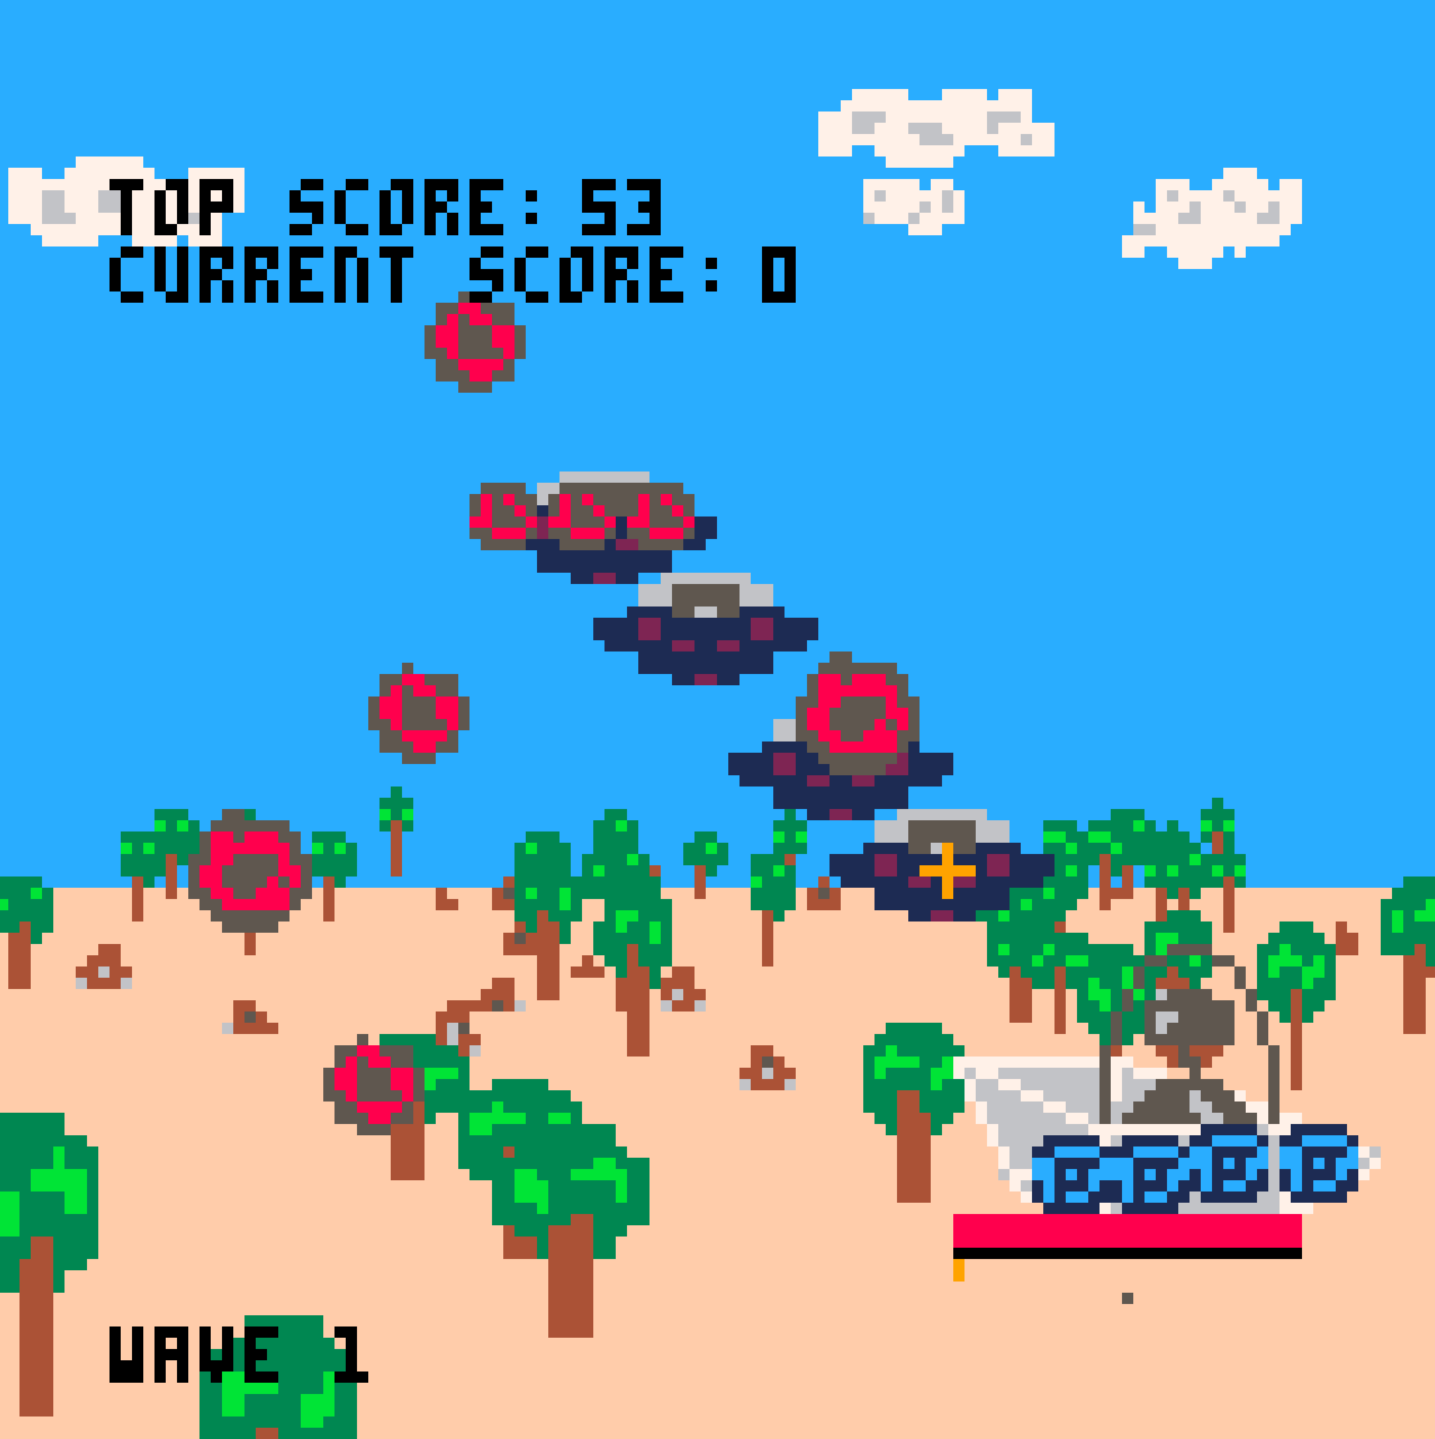
\includegraphics[width=.8\textwidth]{final3d}
    \caption{final software}
    \label{fig:3dfinal}
\end{figure}

\subsection{The update loop}

\subsubsection*{Updating the gameworld}
The given \textunderscore update() loop present in the main game file simply calls one
function: the update() function of the game\textunderscore world table.

First we perform a simple check for player death with a branch that executes if the
life of our player is less than or equal to zero. If this is the case, we check if
the player's current score is higher than the cart's high score, and reassign the
cart's high score in persistent cart data if so. Finally, we pass control back to
the menu cart with a load() call.

If the player has not died, control passes to logic that controls our current enemy
wave. We will discuss the internal functioning of enemy waves below, but at a high level
we check if a wave has been completed and, if so, adjust the global
speed\textunderscore factor of the game as a naive tuner for escalating difficulty
(see Section \ref{tlx} for more information on difficulty scaling).

If a wave has
been completed and we have not reached our maximum number of pre-boss waves,
we initialise a new wave and increment our wave counter - as well as spawning
one of three potential in-game pick-ups to reward players between waves.

If we have reached the final
wave, we instead call a function to store our existing scenery in PICO-8 memory and
make a load() call to run the cart containing our boss encounter (discussed below in
Section \ref{boss}).

After this logic has executed, and assuming we have not loaded the boss encounter
cart, the game will run the update function of its current wave - either deriving
the next frame's worth of activity for our current enemy wave, or else deriving the
first frame's worth of activity for our newly initialised wave.

We then update our player - taking and handling any user input, and testing for
appropriate collisions - before finally managing our scenery, fired projectiles,
and various spawned pick-ups.

\subsubsection*{Updating the current enemy wave}

The wave table's update() method can be broken down neatly into two sections: the first
of which executes the specific behaviour of this class of wave, and the second of
which executes generic updating tasks common to all types of enemy wave present in
the game.

At initialisation, a wave takes one one of four forms depending on the current
game\textunderscore world wave counter. These four forms describe enemy waves in which,
respectively, the incoming enemy ships: are saucers that move in a sweeping motion,
are saucers that move in a circular motion, are saucers that move in a spreading motion,
or are drone enemies who attack the player in a ``Kamikaze'' fashion.

Once initialised - ie, once the newly created table has been set to one of these
four modes, each with a unique internal update - the wave, once updated by the
game\textunderscore world update() function, will call its own internal
class\textunderscore update() method in order to execute the behaviour of one of
the four subtypes. This largely consists of timer-based control over the spawn of
enemies up to a limit.

Once this class\textunderscore update() is complete, the wave table carries out
more generalised hygiene on the enemies it contains.

Firstly, the update() method iterates through the enemies it contains and
checks whether or not they were marked as destroyed during the previous frame.
If so, a new explosion is initiated at their current position and they are
subsequently removed from the list of enemies - along with a point of score being
awarded to the player and a simple explosion sound effect being called.

Then, enemies are tested for position - if they have moved behind the viewport,
they are considered off-screen and are removed from the wave's table of enemies.
Since we define the behaviour of enemies and have determined that they move
contrarywise to the player at all times, we can safetly assume that they will
not return.

We then iterate through the wave's table of ongoing explosions, and remove those
that have expired (ie, their internal counter has reached zero).

Once that has been done, we update first all of our enemies and then all of
our explosions. The enemy update() function will be discussed below. The
explosion update() function is significantly simpler and broadly executes
the animation logic of progressive sprite expansion and quasi-random flipping
outlined in Section \ref{conversion}.

Once all enemies and explosions have been updated, we make a final check to
see if the wave has been completed - that is, that the wave has persisted for
more than 300 frames or ten seconds (the chosen time window across which a
wave will spawn its enemies) and there are no enemies or explosions remaining.
If so, the wave is marked as completed and the game\textunderscore world update()
function will initialise a new one in the next frame as discussed above.

\subsubsection*{Updating individual enemies}

Discuss the update operations of individual enemies including bullet collision checks, movement, and
timed firing. Discuss consequence of bullet collision, and creation of explosion objects - referring back
to prior section outlining the implementation of the explosion animation and particle effect. Discuss
the decision to use sequential rather than simultaneous movement, its drawbacks, and its suitability for
a video game system.\cite[p. 16]{ericson}

\subsubsection*{Updating the player}

Blah blah.

\subsubsection*{Suitability of fixed step updating in PICO-8}

As mentioned in Section \ref{pico}, one of the major advantages of PICO-8 as a development platform
is its portability and low demands on hardware, virtually guaranteeing a stable rate of performance
that effectively emulates the targetted compute power. As such, we are working with a relatively fixed
frame budget and can program accordingly, eschewing more complex patterns intended to stabilise
game persistence across multiple hardware configurations of differing capability.

To quote former Electronic Arts developer Robert Nystrom\cite[p. 126]{nystrom}, ``few developers have
the luxury of knowing exactly what hardware their game will run on. Instead, our games must intelligently
adapt to a variety of devices.'' PICO-8 is very much an exception to this rule, since any reasonable
hardware variation will not impact the game speed if properly budgeted, and as such approaches like
variable time step updating or variable rendering are irrelevant to our concerns. Naive fixed-step updating
is reasonable in this context, and more complex approaches would be over-engineered - in addition to eating
valuable token space.

Discuss player input scheme with particular reference to lock-on system.

Discuss scenery, bullet, and pick-up management. Justify timing of bullet update and outline alternative
approaches \cite{nystrom}.
\subsection{The draw loop}

Unlike the \textunderscore update() function, our drawing function contains two function calls - the first of which
draws the game world in its entirety (which is the lion's share of the work) and the second of which
draws a minimal Heads Up Display (HUD) over it, aligned to our player ship. We will discuss each on turn
and also briefly discuss the lack of a need for a bespoke implementation of double frame buffering.

\subsubsection*{Drawing the game world}
Discuss the initial drawing of a flat surface using rectfill() and its population by scrolling scenery.
Discuss the design decisions behind the use of trees, rocks, and clouds and their ability to be easily
rotated without jarring consequence. Discuss positioning of scenery outside the effective range of
play, and why this makes it appropriate to draw static scenery first.

Discuss the use of the z-sort algorithm to correctly order sprites and polygonal objects
for correct ordering by depth. 

Refer to earlier 3D projection discussion and discuss how this is used as the foundation for
spriteobject level draw calls that use object-level sprite-sheet data.

Discuss the use of pal() calls to simulate lights and rotary blades in the saucer and drone
enemies.

Discuss the use of backface culling for the player ship and the decision to draw backfaces
within the boss, allowing for the use of a hollow ``shell'' shape to enhance gameplay.

Discuss the use of recoloured sprites and semi-random sprite flipping to draw player thrusters
with a dynamic quality.

% Discuss the in-game HUD. Trace its development from the initial software prototype, its brief
% abandonment, and its reintroduction following user testing feedback about the failure of players
% to engage with more traditional HUD elements on the borders of the display.

\subsubsection*{Drawing the HUD}

After the game world has been ordered for depth and drawn as described above, the in-game Heads Up
Display (HUD) is drawn over the scene. Two alternative approaches to designing this element were
taken and the decision between them vacilated over the course of the project.

The first and most obvious approach was to display pertinent information - such as player health,
a target acquired count, and a lock-on cooldown - on the edges of the screen, as is traditional in
many third person action games. At the end of the prototyping phase an alternative approach was
briefly taken, in which information was displayed within the game world as an accompaniment to
the player ship model. The initial implementation of this was misguided, and worked by projecting
HUD elements along with the ship, creating rotational distortion that made the information difficult
to read and distracting.

Following reversion to a more traditional HUD, the decision was again taken to re-implement a
HUD that followed the player ship - except this time drawn straightforwardly in screen space
rather than projected with the ship itself. This decision was taken during think aloud user testing,
during which several participants reported an inability or unwillingness to track peripheral
information while focusing on the core aim-and-shoot activity of the game.

\subsubsection*{A note on PICO-8 and double buffering}

As discussed above with regards to the update loop and the viability of fixed-step updating given
the performance profile of PICO-8, we also do not need to concern ourselves here with programming
patterns that eliminate screen tearing and other graphical artefacts. PICO-8 uses a form of double
buffering internally which produces smooth screen drawing without the developer needing to worry about
bespoke implementation - all video memory is updated simultaneously at the conclusion of the
in-built \textunderscore draw() function. As such, well understood patterns like double
buffering\cite[p. 107]{nystrom} do not need to be re-implemented by the developer.

\subsection{Transition to multi-cart design}\label{multicart}
% Discuss late impact of token limit. Discuss decision to eschew imposed limitation of
% PICO-8 and convert game to a multi-cart project. Discuss benefits of approach, including
% introduction of straightforward game start/game over/restart logic based on storage of
% pertinent persistent data and use of cart reloading. 

One late decision taken, following an encounter with the token limit of a single PICO-8 cart
in the development of the game's boss encounter (discussed below in Section \ref{boss}), was to
split the game across multiple carts.

The game is initially run through a main cart that contains the logic and data required to
run the core gameplay loop outlined above. Once the final wave of normal gameplay is cleared,
the game runs a load() and run() command on an additional cart containing the boss mode - which
shares much data and functionality with the main game cart, but also strips out extraneous
code describing certain enemy behaviours that don't appear in the boss encounter in favour of
code describing the logic of the boss.

% ELIMINATE IF CANNOT FIX IN GAME
In order to ensure continuity between carts, certain data is stored in system storage before
the load() and run() commands are run and then read by the new cart on initialisation, allowing
the creation of consistent scenery density and placement between loads.

% REWORK THIS PARAGRAPH SIGNIFICANTLY
Furthermore, logic controlling the broader game system - such as restarts and game over screens -
is outsourced to an additional cart for simplicity, avoiding the token burden of including this
logic in the main cart and simplifying the procedure for restarting the game through cart reloading
(with persistent state stored using PICO-8's in-built facilities) rather than through more
comprehensive state resetting in code.

\subsection{Boss mode}\label{boss}

\begin{figure}[h]
\begin{subfigure}{.5\textwidth}
  \centering
  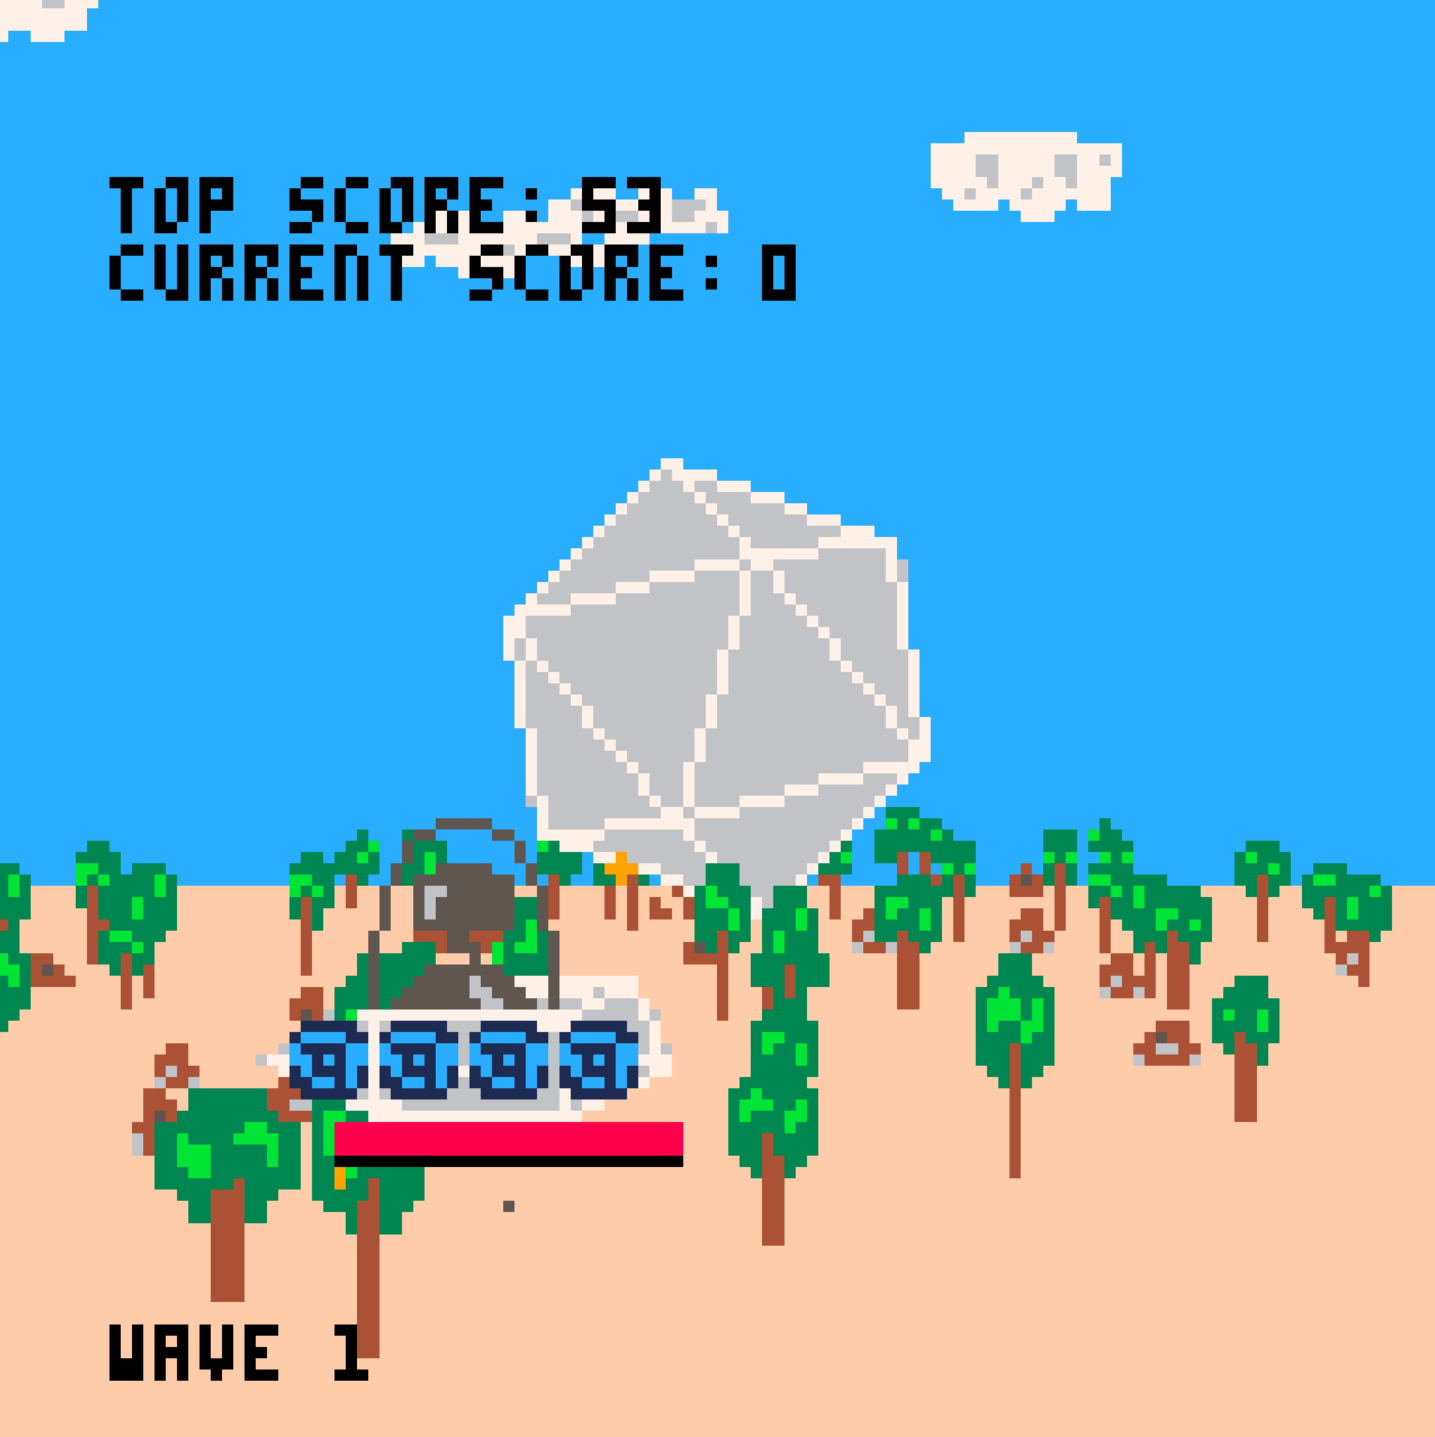
\includegraphics[width=.8\linewidth]{boss1}
  \caption{boss mode approach}
  \label{fig:bossfig1}
\end{subfigure}\hfill
\begin{subfigure}{.5\textwidth}
  \centering
  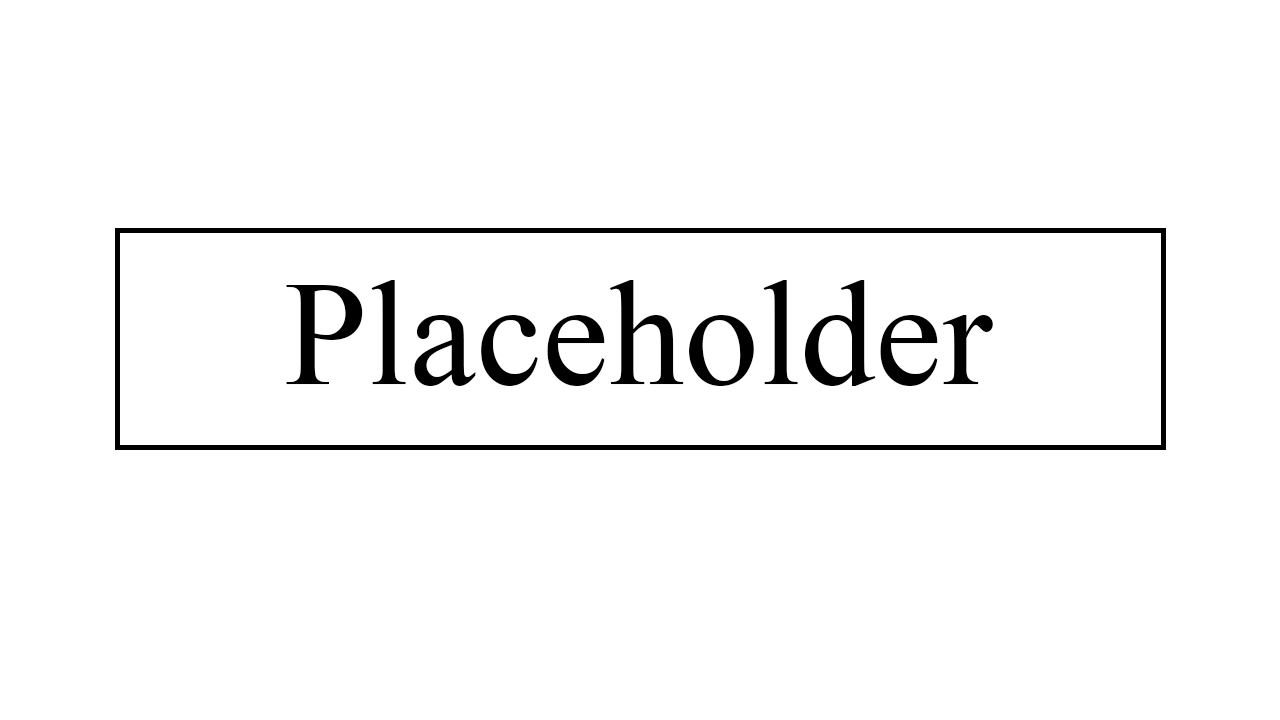
\includegraphics[width=.8\linewidth]{placeholder}
  \caption{boss mode gameplay}
  \label{fig:bossfig2}
\end{subfigure}\hfill
\caption{boss mode}
\label{fig:boss}
\end{figure}

% Discuss thinking behind 3D boss design - with emphasis on opportunity to explore additional way to
% navigate 3D space with similar constraints to rail shooter genre. Compare to boss set-pieces in
% \textit{Panzer Dragoon} and \textit{Rez}.

Having implemented a core gameplay loop executing on the basic gameplay of the rail shooter genre,
development began on a climactic boss battle. Bosses in rail shooters have historically taken many
forms and suggest multiple alternative approaches - here we will briefly consider a few early
bosses from genre exemplars. 

In \textit{Space Harrier}, the player is confronted with a dragon composed of multiple
repeated sprites to represent a body, and a additional sprites to represent the head and the
point of a tail. These sprites are drawn in different orders to represent backwards and forwards
movement, and the player defeats the boss by inflicting repeated damage and reducing its size.

In \textit{Panzer Dragoon}, a more complex set piece is established in which the player (riding a 
dragon) navigates around a hostile ship in a circle - using camera controls discussed in Section
\ref{genre} and attacking turrets and other discrete parts of the ship's body.

In \textit{Rez}, the player circles around a spherical hollow shell composed of numerous discrete
faces, which they must shoot open in order to attack a point within before the shell is rebuilt.

In order to exploit built functionality for polygonal rendering and the rotation of polygonal
models - previously reserved for rendering a player ship - it was decided to opt for a boss
design more akin to \textit{Panzer Dragoon} and \textit{Rez} that worked on the principle of
circular motion around a point and the progressive destruction of a shell.

\subsubsection*{Camera rotations in 3D space}

% Discuss the implementation of camera rotations around a point in 3D space for the
% creation of a ``boss mode'' which involves strafing around a polygonal enemy. 

In order to execute on this concept, a new camera mode had to be built for the game.
Whereas the general course of play sees the camera in a fixed position at origin, looking
along the \textit{z}-axis while enemies and geometry scroll towards it and the player
model moves in a fixed two-dimensional plane parallel to the viewport, a boss setpiece in
which the player ship strafes around a polygonal enemy required the camera to sweep in a 
circle around the boss.

Camera transformations, in this implementation, work on the principle that real camera
transformations and the application of contrary transformations on scenery objects
produce like results. As such, as illustrated in Figure \ref{fig:rotation}, camera transformations
in this mode are accomplished by transforming world scenery to simulate the movement of the camera.

In this example, to rotate objects in a scene around an arbitrary point, the objects are
translated by the inverse of the position vector of the point of rotation, rotated around
origin, and translated by by the positive position vector of the initial point.

As implemented in the game, this means that objects in the game world are rotated around
the position of the boss - at coordinates (0, 0, 5) - in the opposite direction to the
putitive movement of the camera as generated by player input, in order to generate the
phenomeon of a camera sweeping through space.

\begin{figure}[h]
\begin{subfigure}{.45\textwidth}
   \centering
   \begin{tikzpicture}
      [scale = 2,
      axis/.style={-stealth},
      dot/.style= {
         draw,
         fill = black,
         circle,
         inner sep = 0pt,
         minimum size = 4pt
      },
      point/.style= {
         draw,
         fill = black,
         circle,
         inner sep = 0pt,
         minimum size = 2pt
      }]
      
      \draw[axis] (-1.25, 0) -- (1.25, 0) node[right] {$x$};
      \draw[axis] (0, -1.5) -- (0, 1.5) node[above] {$z$};

      \draw (0.5, 0.5) node[dot, label = {above:$r$}] {};
      \draw [black, ->] (0.5, 0.5) -- (0, 0);

      \draw (-0.3, 0.6) node[point, label = {above:$o_1$}] {};
      \draw [gray, ->] (-0.3, 0.6) -- (-0.8, 0.1);
      \draw (-0.8, 0.1) node[point, label = {above:$t_1$}] {};

      \draw (0.9, 0.2) node[point, label = {above:$o_2$}] {};
      \draw [gray, ->] (0.9, 0.2) -- (0.4, -0.3);
      \draw (0.4, -0.3) node[point, label = {above:$t_2$}] {};

      \draw (-0.4, -0.4) node[point, label = {above:$o_3$}] {};
      \draw [gray, ->] (-0.4, -0.4) -- (-0.9, -0.9);
      \draw (-0.9, -0.9) node[point, label = {above:$t_3$}] {};

   \end{tikzpicture}
   \caption{select point \textit{r} in 2D plane around which to rotate scene, and translate
   all objects \textit{o} by the inverse of its position vector to positions \textit{t}}
   \label{fig:rotfig1}
\end{subfigure}\hfill
\begin{subfigure}{.45\textwidth}
   \centering
   \begin{tikzpicture}
      [scale = 2,
      axis/.style={-stealth},
      dot/.style= {
         draw,
         fill = black,
         circle,
         inner sep = 0pt,
         minimum size = 4pt
      },
      point/.style= {
         draw,
         fill = black,
         circle,
         inner sep = 0pt,
         minimum size = 2pt
      }]
      \draw[axis] (-1.25, 0) -- (1.25, 0) node[right] {$x$};
      \draw[axis] (0, -1.5) -- (0, 1.5) node[above] {$z$};

      \draw (0.5, 0.5) node[dot, label = {above:$r$}] {};

      \coordinate (R) at (0.5, 0.5);

      \pgfmathsetmacro{\angle}{70}
      \pgfmathsetmacro{\tx}{-0.8}
      \pgfmathsetmacro{\ty}{0.1}
      \coordinate (t1) at (\tx, \ty);
      \pgfmathsetmacro{\rx}{\tx*cos(\angle) - \ty*sin(\angle)}
      \pgfmathsetmacro{\ry}{\tx*sin(\angle) + \ty*cos(\angle)}
      \pgfmathsetmacro{\radius}{sqrt((\tx * \tx) + (\ty * \ty))}
      \coordinate (r1) at (\rx,\ry);
      \draw (t1) node[point, label = {above:$t_1$}] {};
      \draw (r1) node[point] {};
      \begin{scope}
         \clip (-1, \ty) rectangle (0, \ry);
         \draw[densely dotted] circle(\radius);
      \end{scope}
      \draw [gray, ->] (r1) -- ($(r1)+(R)$);
      \draw ($(r1)+(R)$) node[point, label = {above:$p_1$}] {};

      \pgfmathsetmacro{\tx}{0.4}
      \pgfmathsetmacro{\ty}{-0.3}
      \coordinate (t2) at (\tx, \ty);
      \pgfmathsetmacro{\rx}{\tx*cos(\angle) - \ty*sin(\angle)}
      \pgfmathsetmacro{\ry}{\tx*sin(\angle) + \ty*cos(\angle)}
      \pgfmathsetmacro{\radius}{sqrt((\tx * \tx) + (\ty * \ty))}
      \coordinate (r2) at (\rx,\ry);
      \draw (t2) node[point, label = {above:$t_2$}] {};
      \draw (r2) node[point] {};
      \begin{scope}
         \clip (1, \ty) rectangle (0, \ry);
         \draw[densely dotted] circle(\radius);
      \end{scope}
      \draw [gray, ->] (r2) -- ($(r2)+(R)$);
      \draw ($(r2)+(R)$) node[point, label = {above:$p_2$}] {};

      \pgfmathsetmacro{\tx}{-0.9}
      \pgfmathsetmacro{\ty}{-0.9}
      \coordinate (t3) at (\tx, \ty);
      \pgfmathsetmacro{\rx}{\tx*cos(\angle) - \ty*sin(\angle)}
      \pgfmathsetmacro{\ry}{\tx*sin(\angle) + \ty*cos(\angle)}
      \pgfmathsetmacro{\radius}{sqrt((\tx * \tx) + (\ty * \ty))}
      \coordinate (r3) at (\rx,\ry);
      \draw (t3) node[point, label = {above:$t_3$}] {};
      \draw (r3) node[point] {};
      \begin{scope}
         \clip (t3) rectangle (\rx, -1.5);
         \draw[densely dotted] circle(\radius);
      \end{scope}
      \draw [gray, ->] (r3) -- ($(r3)+(R)$);
      \draw ($(r3)+(R)$) node[point, label = {above:$p_3$}] {};

   \end{tikzpicture}
   \caption{rotate translated points \textit{t} around (0, 0) and translate them again by positive
   position vector of chosen point of rotation to find final position \textit{p}}
   \label{fig:rotfig2}
\end{subfigure}\hfill
\caption{\textit{y}-axis rotation of a scene around an arbitrary point in 3D space}
\label{fig:rotation}
\end{figure}

% Highlight the implications of this change on the position and orientation of the player model,
% which can no longer exist naively in a 2D plane facing along the z-axis but which
% must now be able to exist in a rotational relationship to a focal point in the map,
% shared with the camera.

This change also forced reconsideration of how the position of the player is defined
in the game world, and associated issues such as direction of fire. Whereas the position
of the player ship had previously been defined as a point in 3D space confined to a 2D
plane parallel to the camera viewport, free-firing projectiles directly down the \textit{z}-axis,
strafing motion around a stationary boss setpiece required the position of the ship to instead
be defined by an angle around a unit circle.

Two alternative approaches to free-firing under this new approach were considered. Firstly,
the technically correct approach, would see the ship firing directly forward as it faced - with
the unfortunate implication that all shots would ultimately travel through the centre of
rotation, and thus cause undue constraint on player action. The alternative, which was adopted,
saw the ship maintain its freedom to fire from arbitrary points on a 2D plane by directing
bullets down the direction faced by the camera rather than the player ship - a trade-off
that favoured game feel over accurate simulation.

% Discuss the relationship between in-frame player movement,
% the implied field of view of a 1x1 canvas at single unit distance from pinhole, and
% camera rotation around a point. Discuss the per-object rotations required to execute
% such camera movements, density of spawned scenery, and concerns around computational
% load.

\subsubsection*{Ray-triangle collision with the Möller–Trumbore algorithm}

% Discuss the need for more complex ray-triangle intersection computations to effectively
% test for collisions around the boss enemy, since the intended design requires per-face
% collision detection on a regular icosahedron whose faces cannot be satisfactorily
% split into non-overlapping cuboid bounding volumes that adequately approximate
% collisions.

Because the hollow boss enemy shell is composed of twenty triangles forming a regular icosahedron,
and each of the individual triangles needed to be individually destructible, the simple hitbox
approach outlined in Section \ref{conversion} was not sufficient to correctly model the intended
behaviour of the game. As such a more complex collision detection algorithm was required, capable
of handling collisions between moving points (in-game projectiles) and triangles in 3D space.

The implementation of the collision detection algorithm is excerted in Figure \ref{fig:codemoller}, and is
directly adapted from the C++ published in \cite{möller–trumbore}.

\begin{figure}[h]
   \begin{lstlisting}
bullet_triangle_intersect = function(self, bullet, triangle)

   epsilon = 0.0001

   vert0 = self.current_vertices[triangle[1]]
   vert1 = self.current_vertices[triangle[2]]
   vert2 = self.current_vertices[triangle[3]]

   edge1 = subtract(vert1, vert0)
   edge2 = subtract(vert2, vert0)

   pvec = cross_product({bullet.x_increment, bullet.y_increment, bullet.z_increment}, edge2)

   det = dot_product(edge1, pvec)

   -- only use non-culling branch from paper, since boss shell is hollow and can be shot through
   if det > -epsilon and det < epsilon then return false end

   inv_det = 1 / det

   tvec = subtract({bullet.x, bullet.y, bullet.z}, vert0)
   u = dot_product(tvec, pvec) * inv_det
   if (u < 0 or u > 1) then return false end

   qvec = cross_product(tvec, edge1)
   v = dot_product({bullet.x_increment, bullet.y_increment, bullet.z_increment}, qvec) * inv_det
   if (v < 0 or u + v > 1) then return false end

   t = dot_product(edge2, qvec) * inv_det

   if t <= 1 then return true else return false end

end
   \end{lstlisting}
   \caption{Möller–Trumbore algorithm for ray-triangle intersections}
   \label{fig:codemoller}
\end{figure}

One limitation of this approach is that projectiles are modelled as points in space rather than
objects with volume, which is contrary to their handling in other game situations, but this
inconsistency was accepted on the previously mentioned principle of ``if it feels right, it is
right'', which is one of the advantages of working in non-critical real time applications -
allowing us to eschew the additional overhead of performing this calculation for the eight vertices
of a cuboid bounding volume, or implementing a more bespoke calculation that accurately tests for
the collision of a triangle with any points on the surface of a sphere.

\section{Results}
\subsection{Think-aloud testing feedback}
Discuss feedback gathered by think-aloud testing sessions, and highlight adaptations
to the software intended to answer constructive criticisms. Possible subjects of
discussion:
\begin{itemize}
   \item implementation of on-player HUD to answer lack of player attention on vital
   gameplay statistics, ie remaining life and state of lock-on targetting;
   \item redesign of pick-up sprites to better differentiate power-ups from
   damage-inducing projectiles;
   \item introduction of narrative splash screen to justify on-screen action, which
   was seen as random and unexplained.
\end{itemize}
Also discuss positive feedback gathered during sessions, such as satisfaction
with the game controls, hit detection, and overall aesthetic of the game, and comfort
with depth perception despite the low-resolution pixel grid.
\subsection{Formal NASA-TLX testing}\label{tlx}
I also subjected my programme to one round of quantitative testing to investigate the
relative contributions of enemy speed and enemy fire rate to overall difficulty - as
measured by task load.

This was done through the use of the widely used and validated NASA-TLX survey on which...

TO DO: GENERAL EXPLANATION OF NASA-TLX

Participants were asked to play three builds of the game - a control build, in which enemy
ships behaved in a ``normal'' way, a rapid fire build in which enemy ships move at a standard
speed but fire more quickly, and a rapid movement build in which the rate of fire is the same
as in the control but the ships move faster.

TO DO: CALCULATE RESULTS OF NASA-TLX SURVEYS TAKEN ON 11/08


\section{Evaluation}
\subsection{Pitfalls of paper prototyping for 3D projects}\label{prototypepitfalls}
Discuss issues raised by developing initial software prototype from a paper prototype
- with emphasis on inate tendancy of paper prototyping to flatten images to a surface,
mask issues relating to depth-in-space, and discourage serious thinking about the
relationship between world-space and screen-space in projects like this.
\subsection{Artificial limits imposed by featly to platform ethos}
Discuss late move to multicart approach and the creative envelope it opened - too late
in the project. Discuss attempts to remain within arbitrary token limit for much of the
project and speculate about additional game modes that could have been introduced hardware
a multicart approach been taken sooner (including both alternative boss designs, more
data-intensive 3D ideas, and variations on the core gameplay loop)
\subsection{Unavoidable limitations imposed by PICO-8}
Discuss issues caused by coarseness of PICO-8 pixel grid and difficulties caused by
limited fixed colour palette of PICO-8, and its impact on effective shading of polygonal
models. Discuss use of music and sound in \textit{Rez} and limitations imposed by PICO-8's
low-fi sound system - with equal recognition of creative limitations of developer.


\section{Further work}

\subsection{Additional testing and mechanical pivots}
% Discuss player disinterest in lock-on and possible alternative arrangements to test
One persistent issue revealed in user testing, that was not adequately handled at the completion of
the project as it exists, was player disinterest in using the given lock-on functionality.

Resolution of this design issue could be informed by a round of additional testing, presenting
alternative mechanics to the lock-on as currently implemented.

One approach, which has the downside
of reducing player agency, is to simply make lock-on mandatory for firing - which is the approach
taken in \textit{Rez}, presumably so that the developer can exercise greater control over the timing
of firing events and better syncronise diagetic sound to the game's techno score.

An alternative approach would be to jettison the lock-on mechanic entirely, in the face of
player disinterest, and replace it with an alternative behaviour for holding to fire - one
suggestion, volunteered by a think-aloud tester, was to replace this mechanic with a weapon
charging mechanic, allowing players to fire off more or less powerful free shots by holding
the input for more or less time. This would pose the additional problem of either adding
additional information to the HUD in order to illustrate charge level, or else to rely on
player intuition and risk creating a false feeling of uncertainty.

\subsection{Additional mode development}

Following the switch to a multicart design late in the project, one obvious path for future
development is the exploration of additional gameplay modes that were originally considered
out of scope due to the token limit constraint that exists with single cart PICO-8 games.
Here I will briefly discuss some game modes that could be straightforwardly implemented
given functionality that has already been built to rotate our camera around arbitrary
points in 3D space.

\begin{figure}[h]
\begin{subfigure}{.45\textwidth}
  \centering
  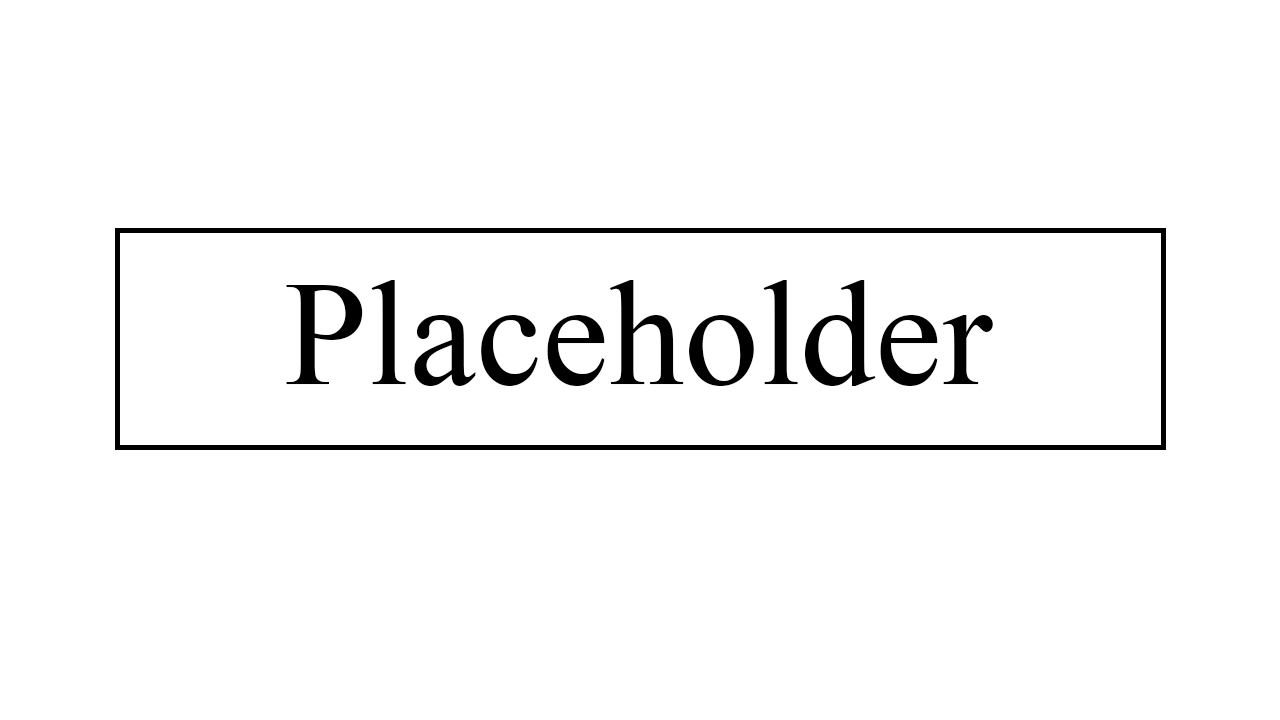
\includegraphics[width=.8\linewidth]{placeholder}
  \caption{an example of side-on action in \textit{Rez Infinite}}
  \label{fig:sideways}
\end{subfigure}\hfill
\begin{subfigure}{.45\textwidth}
  \centering
  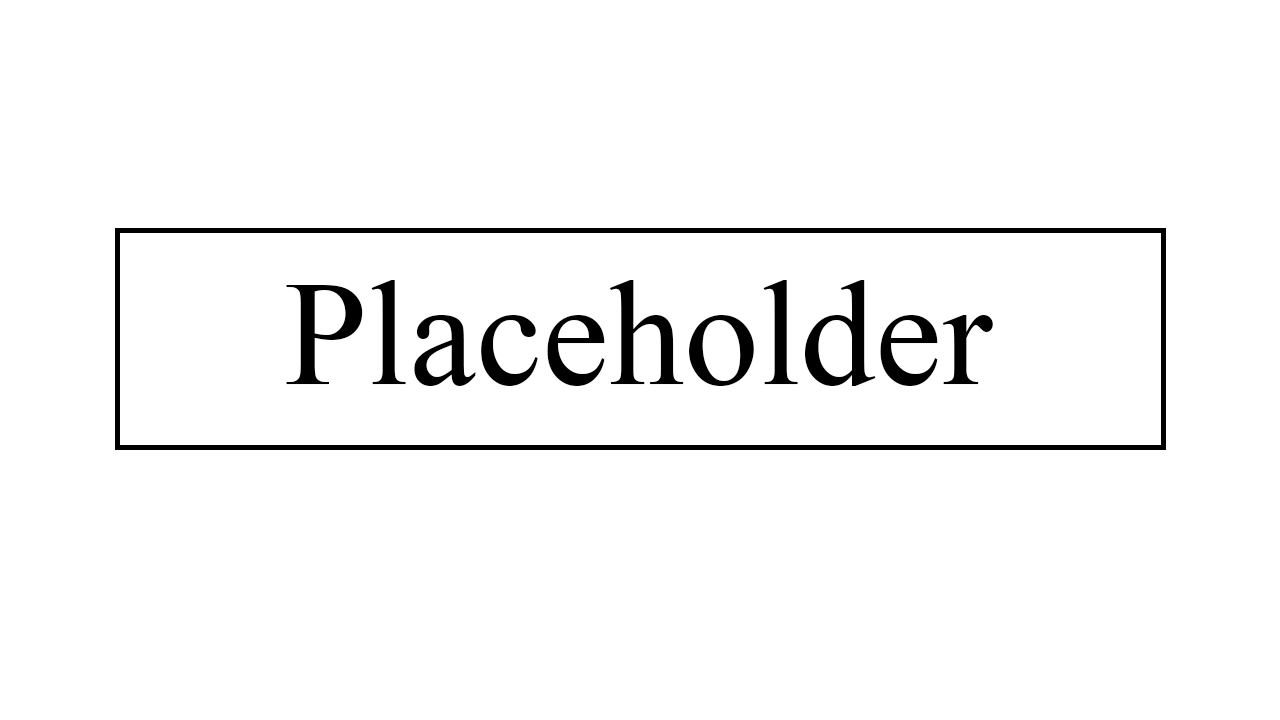
\includegraphics[width=.8\linewidth]{placeholder}
  \caption{an example of shmup gameplay, entered into seamlessly from a traditional rail-shooter section, in \textit{Split Fiction}}
  \label{fig:shmup}
\end{subfigure}\hfill
\caption{additional game mode}
\label{fig:additionalmodes}
\end{figure}

\subsubsection*{Sideways chase}
The first such mode would be a side-on mode in which the player continues to move forward
through space but in which the camera now views the player side-on - changing player directional
inputs from controlling direction in the \textit{x} and \textit{y} planes and instead giving
limited control along \textit{z} and \textit{y}.

This player movement and camera set-up would be combined with an enemy approach along the
\textit{z}-axis, on a parallel plane further along the \textit{x}-axis, resulting in gameplay
broadly similiar to that found in the existing game - except with continuous motion now
simulated along the screen rather than down it.

This is broadly in line with the approach taken in \textit{Rez}, where scripted camera movements
result in side-along gameplay and occasional enemy movement from the rear. Such gameplay also
exists in \textit{Panzer Dragoon}, although it is initiated by the player - who can rotate the
camera to four cardinal positions around the dragon using the Sega Saturn's shoulder inputs.

Such an additional mode would highlight the three-dimensional nature of the game world and
create a dynamic alternative to repeated enemy waves using the same camera set-up.

\subsubsection*{Shmup mode}
Brief explanation of shmups. Discuss affinity between rail shooters and shmups. Describe rail section
of \textit{Split Fiction} and seamless transition between game modes. Discuss feasibility given
existing codebase.

\subsection{Change of technology}\label{engines}

As outlined in Section \ref{pico}, PICO-8 is an excellent prototyping tool. But it is inherently
limited, and one obvious course of future work would be to translate the game to more robust technology
and explore the creative possibilities unlocked by a less constrained development environment - most
notabily in graphical effects and in sound synchronisation.

\subsubsection*{Fully-featured game engine: Unreal, Unity, Godot}
Briefly outline various off-the-shelf 3D game engines. Discuss the pros and cons with working with
established technology including robust systems for handling 3D rendering and camera activity. Discuss
drawbacks of the technology. 

\subsubsection*{Minimal game development library: raylib}
Discuss possible alternative benefits of developing using a minimal library like raylib,
which offers similarly freeform low-overhead development to PICO-8 without extraneous
constraints. Note flexibility of the library and ability to use bindings in a range of
languages rather than just Lua or the specified scripting languages imposed by fully-featured
off-the-shelf game engines.


\section{Conclusion}
[To be outlined and written after composition of rest of main body]

\printbibliography

\end{document}